%Phone 
%open chapters on any page, final removes formatting marks
%avoid conflicts with hyperref by loading before documentclass
\RequirePackage{setspace}

\documentclass[11.75pt,openany,final]{memoir}
\makepagenote
\title{The Discoverer's Digest}
%place graphics package first to avoid conflicts (weird page sizes)
\usepackage{graphicx}
\usepackage{wrapfig}

% package to remove 'Figure x.x' with the \caption*{foo} option
\usepackage[labelformat=empty]{caption}

%\usepackage[paperwidth=70.9mm, paperheight=143.6mm, hmargin={1cm, 1cm},vmargin={1.2cm, 1.25cm}]{geometry}
% New setup
% setstocksize{height}{width}
\setstocksize{216mm}{137mm}
\settrimmedsize{216mm}{137mm}{*}
\settypeblocksize{216mm}{137mm}{*}
\setlrmarginsandblock{24.0mm}{24.0mm}{*}
\setulmarginsandblock{27mm}{27mm}{*}
%\marginparmargin{2mm}
% memoir: finalize the page changes
\checkandfixthelayout

\usepackage{microtype}

% \usepackage{marginnote}
%\usepackage{wrapfig}
%\setbeforesecskip{2mm}
% \setaftersecskip{2mm}
%\setSindent{0pt}

% TYPEFACE PROPERTIES
%--------------------
% fontspec system for typeface definitions
\usepackage{fontspec,xunicode,polyglossia}

% Better hanging indent itemize (bullet) list
\usepackage{enumitem}

%NOTE: good discussion of fonts: https://tex.stackexchange.com/questions/352804/setmainfont-vs-fontspec
%letter spacing

%fontspec font selection
%\setmainfont{LinuxLibertineG}[
%BoldFont = LinuxLibertineGB,
%ItalicFont = LinuxLibertineGI,
%BoldItalicFont = LinuxLibertineGZI,
%SlantedFont = LinLibertineSlantedZ,
%BoldSlantedFont = LinLibertineSlantedZ,
%SmallCapsFont = LinLibertineCapitals
%]
\setmainfont{fbb}[%
UprightFeatures = {StylisticSet=01},
BoldFeatures = {StylisticSet=01}
]
\setmonofont{LinLibertine_M}
\setsansfont{LiberationSans}


\makeatletter
%\g@addto@macro\chapnamefont{\sffamily} 
%\g@addto@macro\chapnumfont{\sffamily}  
%\g@addto@macro\chaptitlefont{\sffamily}
%\makeatother

% PAGE PROPERTIES
%----------------
%% common ligatures
%TODO: add more ligatures
\usepackage{newunicodechar}
\newunicodechar{ff}{ff}
\newunicodechar{fi}{fi}
\newunicodechar{fl}{fl}
\newunicodechar{ffi}{ffi}
\newunicodechar{ffl}{ffl}
%% end of common ligatures

% multiple columns (bullet lists, etc.)
\usepackage{multicol}

% set the leading
%better as it leaves margin note spacing alone
\setstretch{1.20}

%flexible margin notes
\usepackage{marginnote}
\renewcommand*{\marginfont}{\color{gray!80!black}\tiny\itshape\setstretch{0.9}}
% End notes
%\usepackage{enotez}
%\setenotez{
%  list-name=Credits
  % split=chapter,
  % split-heading={\chaptermark{#1}}
%}

% CHAPTER PROPERTIES
%-------------------

%chapter page style
\makechapterstyle{plroman}{
\renewcommand\printchaptername{}
\renewcommand\printchapternum{\color{red!70!black}\centering\MakeUppercase{\fontsize{.75in}{1in}\selectfont\romannumeral\thechapter}\color{Black}}
\renewcommand\afterchaptertitle{\vskip0.25\midchapskip\vskip\midchapskip\hrule\vskip0.15\midchapskip\vskip\midchapskip}
}

% Use this chapter style
\chapterstyle{plroman}

% Drop first letter of each chapter
\usepackage{lettrine}

% more text sizes (ssize & HUGE)
\usepackage[10pt]{moresize}

% Precise colors
\usepackage[dvipsnames,svgnames,table]{xcolor}

%story splash images
\usepackage[pages=some,placement=top]{background}

% PDF has priority over PNG (for size reasons) when declaring an extensionless
% \includegraphics
\DeclareGraphicsExtensions{.jpg,.pdf,.png}
%bar
% PAGE HEADER PROPERTIES
% -----------------------
\nouppercaseheads
\makepagestyle{mystyle}
% \makeevenhead{mystyle}{\itshape\thetitle}{}{\scshape\MakeLowercase\rightmark}
% \makeoddhead{mystyle}{}{}{\scshape\MakeLowercase\leftmark}
% page numbers to the inside for easier electronic page number navigation (don't
% need to move eyes back-and-forth)
\makeevenfoot{mystyle}{}{}{\thepage}{}
\makeoddfoot{mystyle}{\thepage}{}{}{}
\makepsmarks{mystyle}{%
  \createmark{chapter}{left}{nonumber}{}{}}

\pagestyle{mystyle}

\usepackage[absolute]{textpos}

% get rid of section period in page header
% \def\sectionmark#1{\markboth{#1}{}}
\def\sectionmark#1{\markboth{#1}{#1}}

% SECTION/SUBSECTION STYLE
% --------------------------
\setsecheadstyle{\color{red!70!black}\Large\scshape\raggedright}
\setsubsecheadstyle{\color{red!70!black}\large\scshape\raggedright}
\setsubsubsecheadstyle{\color{red!70!black}\normalsize\scshape\raggedright}
\setbeforesecskip{-1.5ex plus -.5ex minus -.2ex}
\setaftersecskip{1.3ex plus .2ex}
\setbeforesubsecskip{-1.25ex plus -.5ex minus -.2ex}
\setaftersubsecskip{1ex plus .2ex}

%only use chapters in TOC
\settocdepth{chapter}
\renewcommand{\thesection}{}
\renewcommand{\thesubsection}{}

% USE TIKZ FOR DOT CONVERSION
%(not using this as I converted dot SVG's to PDF)
%\usepackage{tikz}
%\usetikzlibrary{snakes,arrows,shapes}
%\usepackage{amsmath}
\usepackage{lscape}
\usepackage{rotating}

% BETTER REFERENCES
% `on the next page,' etc.
\usepackage{varioref}

% include full-page PDF's
\usepackage{pdfpages}

% source code listing
\usepackage{listings}
\lstset{
  basicstyle=\ssmall\ttfamily,
  columns=fullflexible,
  frame=single,
  breaklines=true,
  postbreak=\mbox{\textcolor{red}{$\hookrightarrow$}\space}
}
\usepackage{parskip}
\setlength{\parindent}{8pt}

% LINK PROPERTIES
%-----------------
\usepackage[pdfversion=1.7,
    pdfauthor={D. Cooper Stevenson},
    pdftitle={The Discoverer's Digest},
    pdfsubject={Interactive Fiction},
    pdfkeywords={Interactive Fiction, Parser, TADS3, Inform, Interactivity},
    pdfproducer={Latex with hyperref},
    pdfcreator={XeLatex}]{hyperref} % Improves typography
\hypersetup{
    colorlinks=true, %Color links instead of ugly boxes
    linkcolor={red!50!black}, %Color of internal links
    citecolor={gray!70!black}, %Color of citations
    urlcolor={red!50!black}, %Color for external hyperlinks
    % urlcolor={BrickRed},
    linktoc=all,
    pdfcenterwindow=true,
  }
\usepackage{attachfile2}
\renewcommand\thefootnote{\textcolor{red!70!black}{\arabic{footnote}}}

\begin{document}
% COVER
%------
%clear the page
\aliaspagestyle{chapter}{empty}

% create a `fake' chapter for title page
\chapter*{}

%define a 'textblock' for the cover image & place image inside cover
\begin{textblock*}{70.9mm}(0mm,0mm)
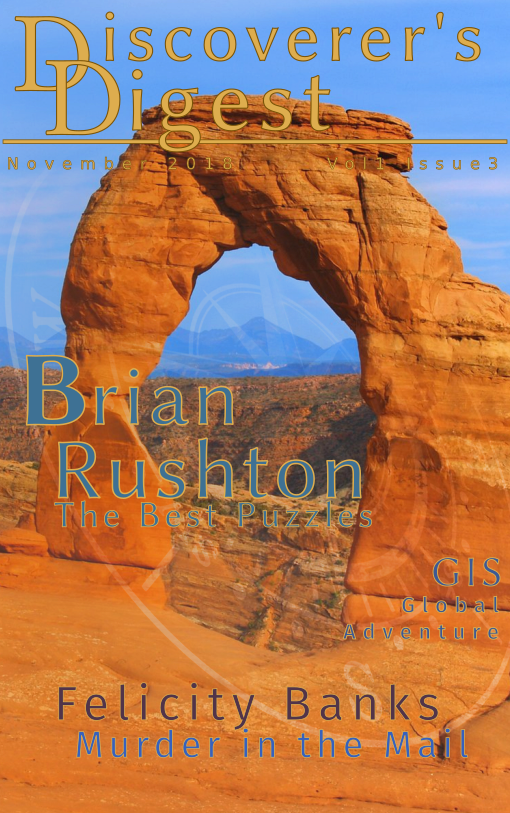
\includegraphics[width=\paperwidth]{./media/images/nov_cover.png}
\end{textblock*}
\thispagestyle{empty}\clearpage %clear header
  %background image for TOC
  \backgroundsetup{
    scale=1,
    color=black,
    %opacity=0.35,
    opacity=0.25,
    angle=0,
    contents={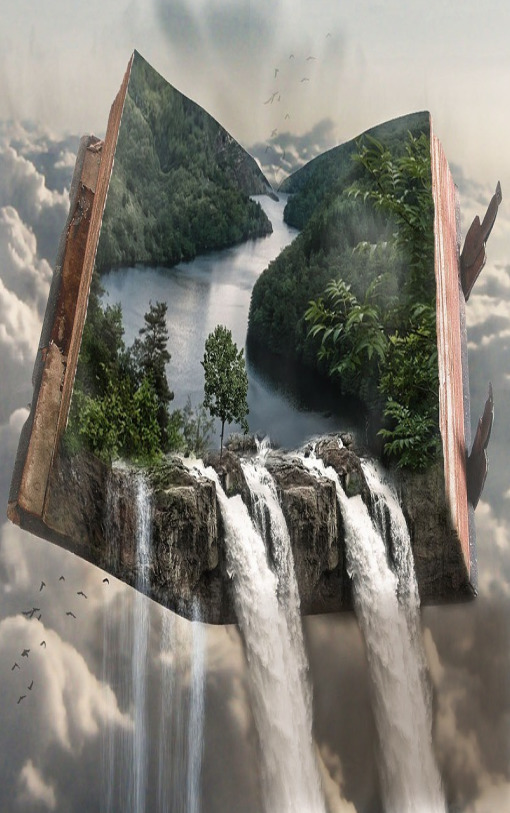
\includegraphics[width=1.01\paperwidth, height=1.01\paperheight,keepaspectratio]{./media/images/cover_splash}}
  }
  \BgThispage
  \tableofcontents*
  \noindent\LARGE{\textbf{Credits}}\medbreak
  \hrule
%  \noindent\rule{9cm}{0.4pt}%watch
  \smallskip
  \noindent\large{\color{red!50!black}{\textbf{Creator\,/\,Graphics\,/\,Author: D. Cooper
        Stevenson}}}\\
  \noindent\small{Cooper Stevenson dedicates himself to enabling fulfilling
    human experiences through the aesthetic use of technology. He lives with his
    wife, \emph{Deanna} and his two cats, \emph{Tiberius} and \emph{Augustus}.}\\ \\
  \noindent\large{\color{red!50!black}{\textbf{Editor: Peter M.J. Gross}}}\\
  \noindent \small{Peter is an editor and online content
  specialist who has been entertained by interactive fiction since "\emph{Nord and
  Bert Couldn't Make Head or Tail of It}." He had to resort to a walkthrough in
  order to complete \emph{Trinity}, and he could never figure out \emph{A Mind Forever
    Voyaging}.}

\thispagestyle{empty} %clear header
\newpage
% First Article
\chapter*{}
\begin{textblock*}{70.9mm}(0mm,0mm)
\includegraphics[width=\paperwidth]{./media/images/editorial_splash}
\end{textblock*}
\clearpage
\chapter{Editorial: Pushing Limits\\ \small{How IF Makes A Difference}}
\begin{figure*}[h]                                                           
 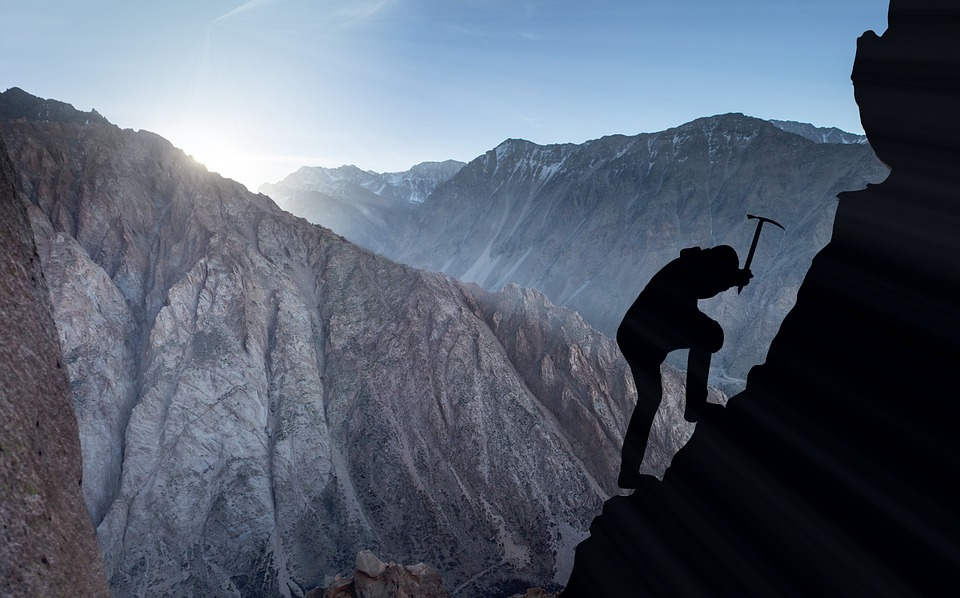
\includegraphics[width=\linewidth]{./media/images/summit}%
%  \scriptsize{\textsc{\\This is} the article main image caption.}
  \label{fig:editorial}%                                                 
\end{figure*}                                                                
\begin{quotation} 
\noindent\color{Sepia}{{\textit{\textbf{“Desire is the starting point of all achievement, not a hope, not a wish, but a keen pulsating desire which transcends everything.”}}}}\\[.5mm]
%remove following line space if you're tight on vertical room and need to fit on
%single page

\hfill\color{Sepia}{\small{\textendash \textsc{Napoleon Hill}}}
\end{quotation} 
\marginnote{Editor's note: margin notes in red signify links pointing to sites of reference}[2em]
%\lettrine[lines=3]{\color{BrickRed}I}{\enspace magine an afternoon outing filled
%  with discovery in detail.} What would it be like to explore a nature trail,
%museum, or even the area around Times Square where each turn presents new
%experiences of the 
\lettrine[lines=3]{\color{BrickRed}L}{\enspace ooking out across Willapa Bay's}
crystal blue waters I wonder about the rich history of this area. Was this
area\textemdash the place I am standing at this moment\textemdash used as a trade
route? Did Native Americans fish here? Could I be standing in the very spot
that a Willapa Chief once surveyed deciding the best course for his people? What
must it be like experiencing this place through the eyes of Natives going back
hundreds of years?

\marginnote{\href{https://en.wikipedia.org/wiki/Chinookan_peoples\#/media/File:Lewis_and_clark-expedition.jpg}{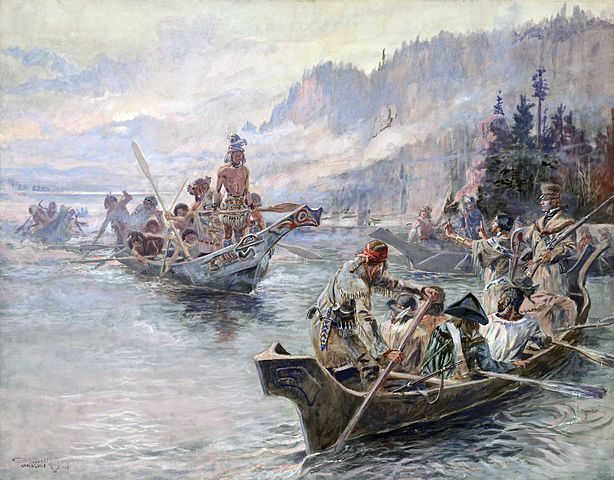
\includegraphics[width=\linewidth]{./media/images/lewis}\\Chinook people meet the Corps of Discovery on the Lower Columbia, October 1805}}[1em]
I approach a little further as my phone vibrates gently letting me know it's 
sensed that I've come to a place having significant import. I read the
Trail Guide's description of the place I am standing with a brief paragraph outlining
that yes, the \emph{Willapa} (or \emph{Willoopah}) tribe, an Northern
Athapaskan\textendash speaking people, did in fact use this very spot as a main
route between the Pacific Ocean 12 miles to the North and the Columbia River to
the South.

I'm no longer just walking along a trail, I'm also walking through time. I close my eyes
and imagine being there when the Chinook people meet the \emph{Corps of Discovery} on the Lower Columbia, near here, in 1805.

\section{limitless exploration}
Continuing along the trail I explore the area's geology, biology, and
wildlife. 
I learn that this area is a critical ``lung'' by which toxins created by water 
runoff is filtered making it
\marginnote{\href{http://portfolio.cooper.stevenson.name/tarlatt/tarlatt_slough_trail_feature_demo.mp4}{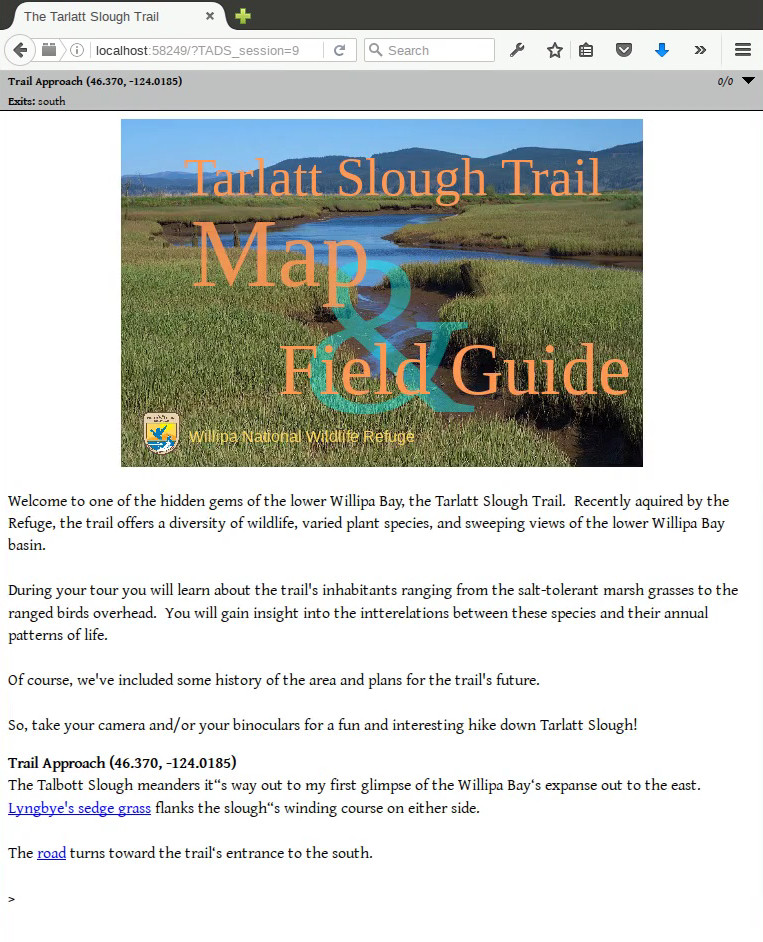
\includegraphics[width=\linewidth]{./media/images/tarlatt}\\Brief
    video showcasing \textsc{gps} enabled Interactive fiction's
    features}}[2em]possible for plankton to thrive giving way to higher forms of wildlife. I learn
that everything I see before me is a delicate balance; I learn of the efforts the
Wildlife Service is performing to keep it that way. I gain a better appreciation
for the area and learn that the term \emph{fragile ecosystem} is more than
mere phrasing; I learn \emph{why}.

\subsection{knowledge you can feel}
\noindent Parents or instructors may afford their children or a group of students impactful
learning experiences through an \texttt{\scriptsize{instructor}} mode (entered as a command
on the parent/instructor's tablet) 
while traveling along with a group of students.
\marginnote{Interlocutors may also \href{https://en.wikipedia.org/wiki/Citizen_science}{participate in Citizen Science} by recording natural findings through the \textsc{if} Tour Guide.}[-3em]
The instructor mode contains
supplemental information to help instructors guide or encourage students to explore areas
that are not obvious. Information imparted by the instructor is heard
by the students \emph{while the students physically interact with the topic at
  hand}. In a single command the instructor or parent is enabled to provide
their students tangible experiences covering a wider range of knowlege with increased depth.  

\subsection{economic benefit}
Interactive tours are not, of course, limited to natural trails. They may be
built for all manner of locations including museum
tours, tourist\textendash based main streets or as a guide for a battlefield
reenactments.
\marginnote{\href{http://www.marshsfreemuseum.com/}{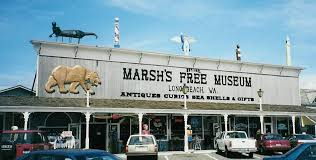
\includegraphics[width=\linewidth]{./media/images/marsh}\\Marsh's
    Free Museum}, in Long Beach Washington, offers all kinds of eclectic stuff including Jake, a
  ``half\textendash man half\textendash alligator.''}
Tourists walking down main street, for example, may learn of the area's
attractions (past and present) just across the street. Long Beach Washington,
for example, features Marsh's Free Museum. Marsh's is, I promise you, is the weirdest
``museum'' you've ever seen. Exhibits include turn\textendash of\textendash
the\textendash century parlor games, live hermit crabs, and ``Jake,'' a (as
legend has it) \emph{real} half\textendash man, half\textendash alligator.
The \textsc{gps\textendash} enabled tour tantalizes the would\textendash be
gawker of all the ridiculous indulgences awaiting inside.

\marginnote{Geocachers may also benefit from \textsc{gps} Interactive Fiction by
having the member solve a brain teaser before revealing the cache's final coordinates}[1em]
Designers can place site\textendash appropriate puzzles in the system for
exploration beyond the physical location. Perhaps an archaeological site is found where the
Interlocutor must figure out how to excavate a precious artifact without
damaging it. For this to work a  particular tool must be found. The reader has
just learned a) the importance of care in archaeology and b) an appreciation for
just how hard the archaeologist's task is. 

Your readers derive added benefit beyond the initial visit and may be passed to
friends and relatives through social media. This encourages others to visit as
the \textsc{if} work offers a preview of the destination from the comfort of
their living room. The shared version of
the work may even
offer embedded advertisements for travel packages and merchandise from the venue
itself or local businesses.

\section{Meaningful Experiences}
This issue if \emph{Discoverer's Digest} explores pushing the limits of
\textsc{if} beyond the screen and parser. The technical guide for enabling
\textsc{gps} in your Interactive Fiction gives a recipee for rich experiences in
the real world by combining the power of an interactive experience with the
sensory awareness of actually \emph{being there}.
\section{the best puzzles}
Brian Rushton systematically breaks down the underlying elements of puzzles
found in Interactive Fiction that help bring enjoyment to the medium. He answers
the questions, ``what are the parameters for good puzzles,'' ``how do I involve
the player,'' and ``what's at stake?''

\section{murder in the mail}
Finally, we've an interview with Felicity Banks, the author of several novels
including \emph{And Their Heroes Were Lost} and \emph{Attack of the Clockwork
  Army}.

Her new work, \emph{Murder in the Mail}, is a feelie story system in which cozy
crime stories are told via physical letters, objects, and high-quality art
prints physically mailed to the reader over several weeks. The reader is invited to guess the identity of the murderer and/or share clues on the forum.

\section{relax and enjoy}
As always, I hope you enjoy this eddition of \emph{Discoverer's Digest}; this
issue looks to be a dandy.

And please submit your news, story ideas, and comments by sending a personal email to \href{mailto:cooper@discdigest.xyz}{cooper@discdigest.xyz}. \\ \\

\noindent Happy Writing! \\ \\

\noindent \href{mailto:cooper@discdigest.xyz}{\textsc{D. Cooper Stevenson}}


\chapter*{}
  \begin{textblock*}{70.9mm}(0mm,0mm)
    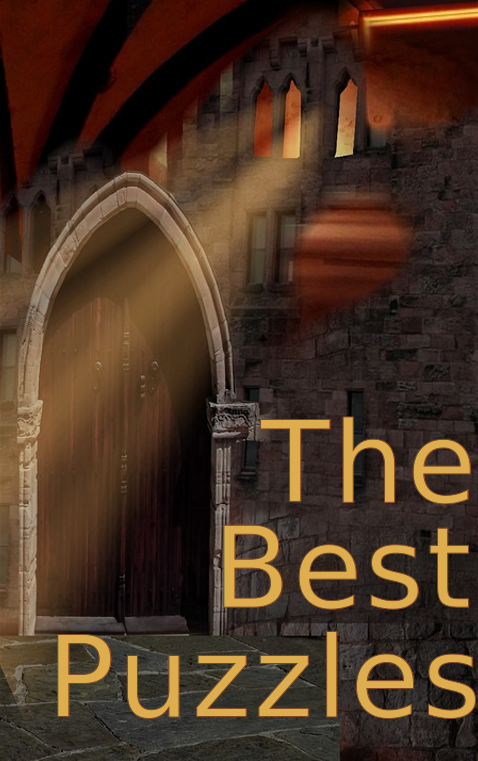
\includegraphics[width=\paperwidth]{./media/images/puzzle_splash}
  \end{textblock*}
  \chapter{The Best Puzzles\\ \small{The Thrill Of Achievement}}
\begin{figure*}[h]                                                           
  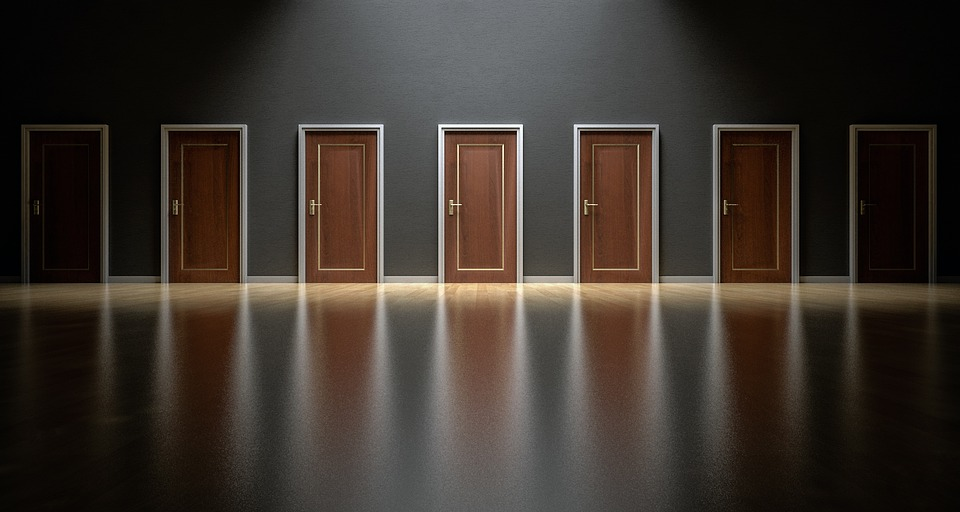
\includegraphics[width=\linewidth]{./media/images/doors}%
%  \scriptsize{\textsc{\\This is} the article main image caption.}
  \label{fig:doors}%                                                 
\end{figure*}                                                                
\begin{quotation} 
\noindent\color{Sepia}{{\textit{\textbf{“Inside of every problem lies an opportunity.”}}}}\\[.5mm]
%remove following line space if you're tight on vertical room and need to fit on
%single page

\hfill\color{Sepia}{\small{\textendash \textsc{Robert Kiposaki}}}
\end{quotation}
\pagebreak
\marginnote{\href{http://ifdb.tads.org/showuser?id=nufzrftl37o9rw5t}{By Brian Rushton}}[2em]
\lettrine[lines=3]{\color{BrickRed}E}{\enspace very year}, voters select one puzzle in one game to receive the \textsc{xyzzy} Best Individual Puzzle Award. These puzzles capture the community’s fancy in some way, through complexity, inventiveness, or even emotion. Of all the \textsc{xyzzy} categories, this award seemed to me like a grab-bag of random games at first, with little connection between different winners.

However, I was determined to find out what they had in common. After carefully playing through all the winning puzzles, I was surprised to find that they fell into a few broad categories. I’d like to discuss these (while avoiding spoilers as much as possible). 

The main categories are Learning a System, Iterative/Babel Fish Puzzles, and Perspective Shift. These categories have some overlap; the Babel Fish puzzles are essentially a blend of the other two categories.

\section{Learning a System}

Roughly half of the best puzzles presented a complex system, sometimes taking up the entire game, which you must learn through experimentation. These puzzles are hard to spoil — your tools and goals are clear from the outset, and the main difficulty is figuring out which tools do what.

The earliest Best Puzzle recipient in this category is the language puzzle in The Edifice (1997), where the player meets an NPC who communicates entirely in a language of the author’s invention. Players must communicate with the NPC and ask specific questions by experimenting with the words they hear.

Another language puzzle appeared in 2001 with The Gostak, a polarizing game that received the IFComp Golden Banana of Discord for having the highest standard deviation in votes. This game is written in a pseudo-English, based on a sentence that says ‘The Gostak distims the doshes’. As in The Edifice, the player must experiment with new words and their responses to learn how to play the game.

The Best Puzzles in 2004 and 2014 involved time travel. All Things Devours (2004) and Fifteen Minutes (2014) are both one-puzzle games with a similar premise: you have run out of time, you have access to a time machine, and more than one version of yourself is required to get the job done. The two games differ in how they handle the multiple versions of yourself. All Things Devours has a large map, and the difficulty in the game is learning how to avoid your copies in order to prevent a paradox from occurring. Fifteen Minutes is a one-room game that relishes having all the copies present and interacting simultaneously. Both games are best approached with copious note-taking materials.

The last two System-Based Best Puzzles are found in Delightful Wallpaper (2006) and An Act of Murder (2007). The first game, by Andrew Plotkin, prevents the player from manipulating anything directly. However, the house they explore reacts to their movement, with movement in one part of the house triggering doors and gates on the other side of the house. The game provides a helpful note-taking system, but it is fiendishly difficult to map out a path that will open the doors you need. The second game, An Act of Murder, is a randomized murder mystery — it also requires careful note-taking to establish alibis and determine motive.

What do these system games have in common? For one, they don’t overwhelm the player. Other attempts at language puzzles dump big dictionaries or convoluted grammar on the player at the start. The Gostak and The Edifice present a sentence or a paragraph and let you go from there. Other time travel puzzles (and there are several of them) can force you to interact with copies of yourself too early.

Conversely, these Best Puzzles also grow complex enough for the player to develop a true feeling of mastery. The Gostak requires a complicated sequence of actions, and the player must make a complicated request in The Edifice. The maze in Delightful Wallpaper was quite large, and the time travel puzzle in Fifteen Minutes can have you interacting with more than half a dozen copies of yourself.

Finally, these puzzles clearly establish the function of each new piece. Delightful Wallpaper will actually write down what you’ve learned at each stage, making it completely unambiguous. The use of each new word in The Gostak or The Edifice is made clear by the many situations it appears in, and so on.

So it appears that people appreciate complicated systems that begin with basic principles and build to a complicated finale. This is the same as learning a system in real life, from mathematics to physics to cooking to speaking a language. These puzzles train you to apply a useful skill (in-game), and they train you well.

\section{Iterative or Babel Fish Puzzles}

The term Babel Fish puzzle comes from the Infocom game Hitchhiker’s Guide to the Galaxy (1984), where the player tried to get a babel fish from a vending machine. When the player fixes the apparent problem preventing them from getting the fish, a new problem is introduced — the fish slips through grates and gets vacuumed up by cleaning robots, but each new failure is only introduced after solving the earlier problems. The term is now used to describe puzzles with an iterative approach, where each new try yields new information.

Puzzles in this category include the games of Rematch (2000) and Lock \& Key (2002), and the sequence in Violet (2008) that disconnects the internet. Some of these could be classified as Learning the System or Perspective Shift puzzles, but I feel they belong here.

Much of the charm in Violet lies more in the writing than in the puzzle structure. Each step makes you laugh at your own lack of self-control, and the counterintuitive actions required for the final solution may color your perception of the central character for the rest of the game.

In Rematch and Lock \& Key, the player sets up a system, sees how it works, and restarts. Rematch is largely about getting a single, complicated command correct — the author warns you that the final command is so long that the parser had to be partially rewritten to accept it. Gameplay consists of iteratively experimenting with lengthier commands until the correct one is found. 

Lock \& Key has you designing a dungeon from about 16 pre-made rooms before watching an adventurer break through them. Like Rematch, it’s clear what each part of the puzzle does, but assembling them in the right order and the right length is difficult. Rematch keeps the puzzle interesting with a super-dramatic recurring event, and Lock \& Key keeps it interesting with hilarious descriptions.

Interestingly, the writing and atmosphere of these puzzles seem to be more responsible for their success than the mechanics of the puzzles themselves. The frequent failures required to advance are shoved in your face, and they are only palatable because of the amusing or compelling messages that you have earned. A Babel fish puzzle without good writing is only an exercise in frustration.

\section{Perspective Shift Puzzles}

These puzzles are difficult to discuss without spoiling, so I’ll talk about them in general terms. They are puzzles where an author has presented the solution, or the puzzle itself, in a deliberately confusing way. You need a sudden flash of insight, usually gained by changing your perspective, to understand the puzzle.

Many authors have tried to write compelling Perspective Shift puzzles and failed. The Best Individual Puzzle winners share a few ingredients to success:
\begin{itemize}[leftmargin=0em]
\item{A constrained environment. In each of these games, the puzzle is solved after almost all other puzzles are out of play, when the player is in a small area and focused on the one puzzle; it is clear that something special is required to move onward.}
\item{The solution involves actions, or clues, that have been introduced earlier. In every case — except perhaps one — an earlier puzzle required you to perform the exact same action for a different purpose. This establishes that the solution is actually possible within the game.}
\item{It involves using something familiar in an unfamiliar way, which is what makes the puzzle interesting.}
\item{Strong dramatic tension adds a sense of urgency to solving the puzzle. This is often the threat of death.}
\end{itemize}
I don’t want to spoil any actual examples, so I’ll use one from literature: in The Fellowship of the Ring, Gandalf and the fellowship must solve a puzzle to open the gates of Moria. Hostile enemies and impassable terrain have closed off their other options. They are in a narrow, dead-end valley that has a lake on one side and the gates on another. 

The inscription on the gates of Moria is originally read as a greeting: “Speak, friend, and enter.” The fellowship spends hours working to identify what needs to be spoken while Gandalf speaks word after word of power.

Finally, with the help of the hobbits, Gandalf laughs and realizes that the inscription is a set of instructions: "Speak 'friend,' and enter.” They speak the word “friend” and open the gates just as a monster attacks.

The characters were in a constrained situation with no other distractions; they had a compelling, story-based need to go in; and the solution was unconventional. The classic idea of a “password” was turned on its head — it was a word that everyone should know, instead of a word that no-one should know. 

The solution was part of the inscription, and there were earlier hints in the book. Much was made of the former friendship between dwarves and elves; the solution supported the earlier information that had been supplied about the old days.

\section{The last puzzle: Four Hats}

The 2011 Best Puzzle is different from the others. Four of the 2011 IFComp games included a recurring character who was looking for his hat. Most people did not notice, or they chalked it up to coincidence (like the year when several games featured a giant squid). 

The four games were quite different: Cold Iron (by an anonymous Plotkin) was a short, mostly puzzle-less story about a world where faeries may or may not exist; Playing Games was a sequence of three mazes made in ASCII art, with a threadbare story tying them together; the Last Day of Summer was a short atmospheric piece about regrets in a village; and the Life and Deaths of Doctor M was a full-blown journey through the afterlife, exploring a doctor’s questionable actions through flashbacks.

All of them had a general setting of late-1800’s to early 1900’s, based on architecture and clothing (for Doctor M, in the afterlife section only), along with a feeling of remembrance and wistfulness. And, of course, the recurring theme of the hat.

The puzzle required information to be transferred between the various games. One game might have something like an opened lock displaying a combination, and the next game has the same combination lock, but closed. One game describes a society where no one talks to you unless you bow three times, and the next game includes that society but doesn’t tell you to bow. You can only see the entire puzzle by playing all 4 games.

I believe that this puzzle won for originality and cleverness; it was a bit unfair in practice. Nobody even deduced its existence during the competition. However, it does have some things in common with the other Best Puzzles: there is a real sense of learning and mastery as you proceed from game to game, because you are applying secret knowledge that is unavailable in the game world. You also use items in unfamiliar ways, providing new perspectives on previously mundane materials. In any case, this is certainly the most unusual of the Best Individual Puzzles.

\section{Conclusion}

While the Best Individual Puzzles are a mixed bag, voters have exhibited some consistent trends. Apart from the hat puzzle, all of the puzzles are fair: either the rules are clearly explained, or the puzzle is set up in a way that allows more than half of the players to stumble onto the solution. All of the puzzles teach the player something, whether a new system or a new way of looking at the game world. 

Each puzzle was also embedded in a polished, bug-free, and frequently well-written game.

What does this mean for authors? It’s hard to come up with specific recommendations, but many authors seem to neglect the idea of fairness. The number of unfair puzzles in games that provide misleading error messages, or provide huge info dumps all at once, or neglect to give any hint as to your purpose, or require you to “guess the verb,” is almost uncountable. 

Ultimately, leading players to a puzzle’s solution seems to require as much
craft as technically implementing the puzzle itself.

\bigskip
\marginnote{\href{http://ifdb.tads.org/showuser?id=nufzrftl37o9rw5t}{Brian
    Rushton's Interactive Fiction Database page}}[1em]
\begin{wrapfigure}{l}{0.25\textwidth}
  \vspace{-3em}
  \begin{center}
  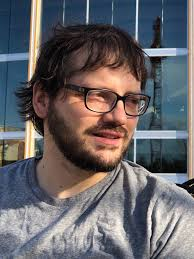
\includegraphics[width=\linewidth]{./media/images/brian}%
%  \scriptsize{\textsc{\\This is} the article main image caption.}
  \label{fig:brian}%
  \end{center}
\end{wrapfigure}                                                                
\noindent\emph{Brian Rushton is a mathematician with an avid interest in interactive fiction.
He currently lives in Washington State with his wife and son, and enjoys stories in every
form. He is also a frequent contributor to the math articles on Wikipedia under
the name \emph{brirush}}.


\chapter*{}
\begin{textblock*}{70.9mm}(0mm,0mm)
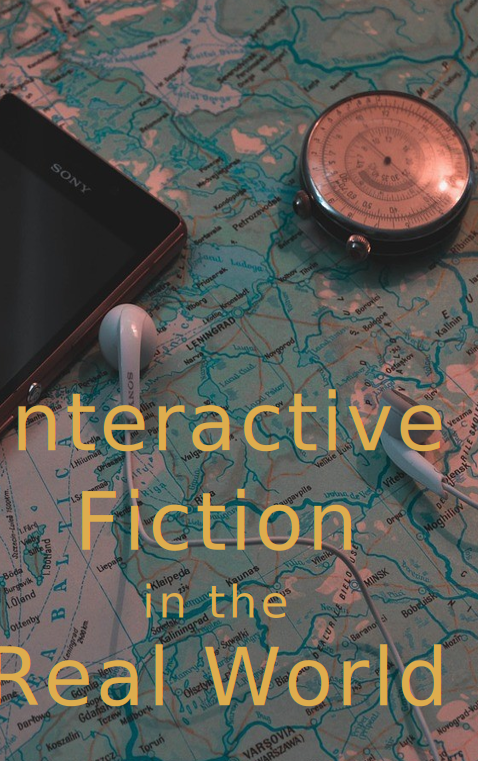
\includegraphics[width=\paperwidth]{./media/images/gps_splash}
\end{textblock*}
\clearpage
\chapter{IF \& GPS\\ \small{Interactive Fiction in the Real World}}
\begin{figure*}[h]                                                           
 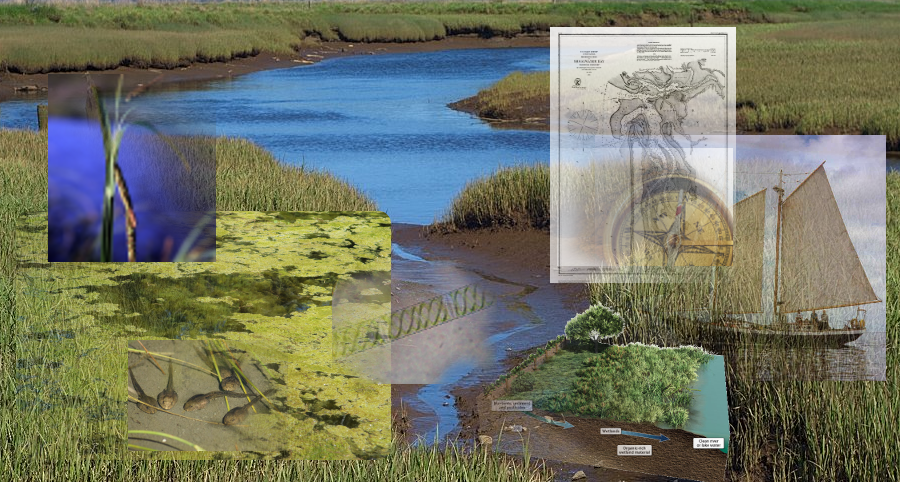
\includegraphics[width=\linewidth]{./media/images/multiple_paths}%
  \scriptsize{\textsc{\\gps enabled interactive fiction} lets your readers explore
  multiple disciplines for a given location including biology, history,
  wildlife, and conservation.}
  \label{fig:multiple_paths}%                                                 
\end{figure*}                                                                
\begin{quotation} 
\noindent\color{Sepia}{{\textit{\textbf{“You never know what's around the corner. It could be everything. Or it could be nothing. You keep putting one foot in front of the other, and then one day you look back and you've climbed a mountain.”}}}}\\[.5mm]
%remove following line space if you're tight on vertical room and need to fit on
%single page

\hfill\color{Sepia}{\small{\textendash \textsc{Tom Hiddleston}}}
\end{quotation} 
\begin{figure*}[h]                                                           
 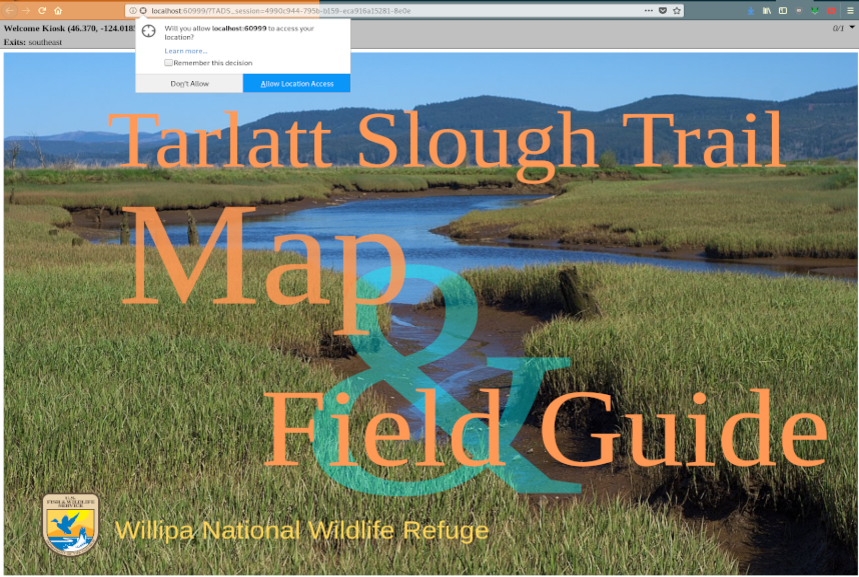
\includegraphics[width=\linewidth]{./media/images/trail_gps.pdf}%
  \scriptsize{\textsc{\\ The user is presented} with a dialog asking for
    permission to access the user's \textsc{gps} device and current location.}
  \label{fig:gps_location}%                                                 
\end{figure*}
This tutorial outlines the build process for creating \textsc{gps} enabled
Interactive fiction. It uses the \textsc{tads3} build system with Javascript
hooks to report \textsc{gps} coordinates from the client's browser to the
Interactive Fiction server.
\marginnote{The compressed version of all the files in the project
  \textattachfile{media/gps.zip}{\color{red!50!black}{\emph{gps.zip}}} (if your PDF
  viewer supports it) is attached here to make it convenient for you to get started}
\noindent Part of \textsc{tads3}'s power lies in it's ability to seamlessly
incluse web objects, styling, and Javascript through the user's browser directly into
your Interactive Fiction. We'll leverage this ability to access the user's
\textsc{gps} sensor to update your story based on the user's current location.
\marginnote{We want to make the experience easy for players not experienced with the parser and thus make heavy use of links}[2em]
The Javascript embedded in the \textsc{tads3} system polls the \textsc{gps}
device every five seconds to see if the traveler has come 
within approximately 10 meters of a known location. When the system detects a
user's new programmed location it will (optionally) send an alert and
automatically update the user's display with a description of their new
surroundings.

Exploration may be had by entering text directly into the parser or through
links embedded in the text so that the traveler need only click on a link to
learn more.

\subsection{prerequisites}
\noindent Creating a workable system requires only that you have a working
\textsc{frobtads} installation. These instructions assume a working Linux installation though they may be easily
adapted to either the Macintosh or Windows platforms. The difference between the
Windows and the Linux and Mac platforms lies largely in the latter two's lack of graphical user
interface. Depending on your development style you may consider the
console\textendash based environment a feature.
\marginnote{The \href{http://www.tads.org/tads3.htm}{\textsc{frobtads } download page}
  makes downloading \textsc{frobtads} easy for your platform. The
  \href{https://github.com/realnc/frobtads}{\textsc{frobtads} repository 
    distribution} is also available for compiling \textsc{frobtads} from the
  latest source.}[-8em]

Once you've finished installing \textsc{frobtads} you can test your installation
by executing the \texttt{t3make} command on the command line. If you receive the
command's help message you've correctly installed the compiler. You can further
test the \textsc{frob} interpreter by entering the \texttt{frob} command on the
command line; you should be greeted with \textsc{frob}'s help message.
\subsection{install generator-tads}
Generator Tads makes it easier to start new projects as it will automatically
create a complete \textsc{tads3} project after answering a few questions about
your project. The template comes complete with build environments for both the
web and terminal versions of your work of \textsc{if}. \textsc{generator-tads}
requires \textsc{nodejs} and \textsc{yeoman} to work.
\subsection{install Yeoman}
\begin{lstlisting}
sudo npm install -g yo
...
Running sanity checks on your system

✔ Global configuration file is valid
✔ NODE_PATH matches the npm root
✔ Node.js version
✔ No .bowerrc file in home directory
✔ No .yo-rc.json file in home directory
✔ npm version
✔ yo version

Everything looks all right!
+ yo@2.0.5
\end{lstlisting}
\marginnote{\href{https://www.anthonyirwin.com/generator-tads/}{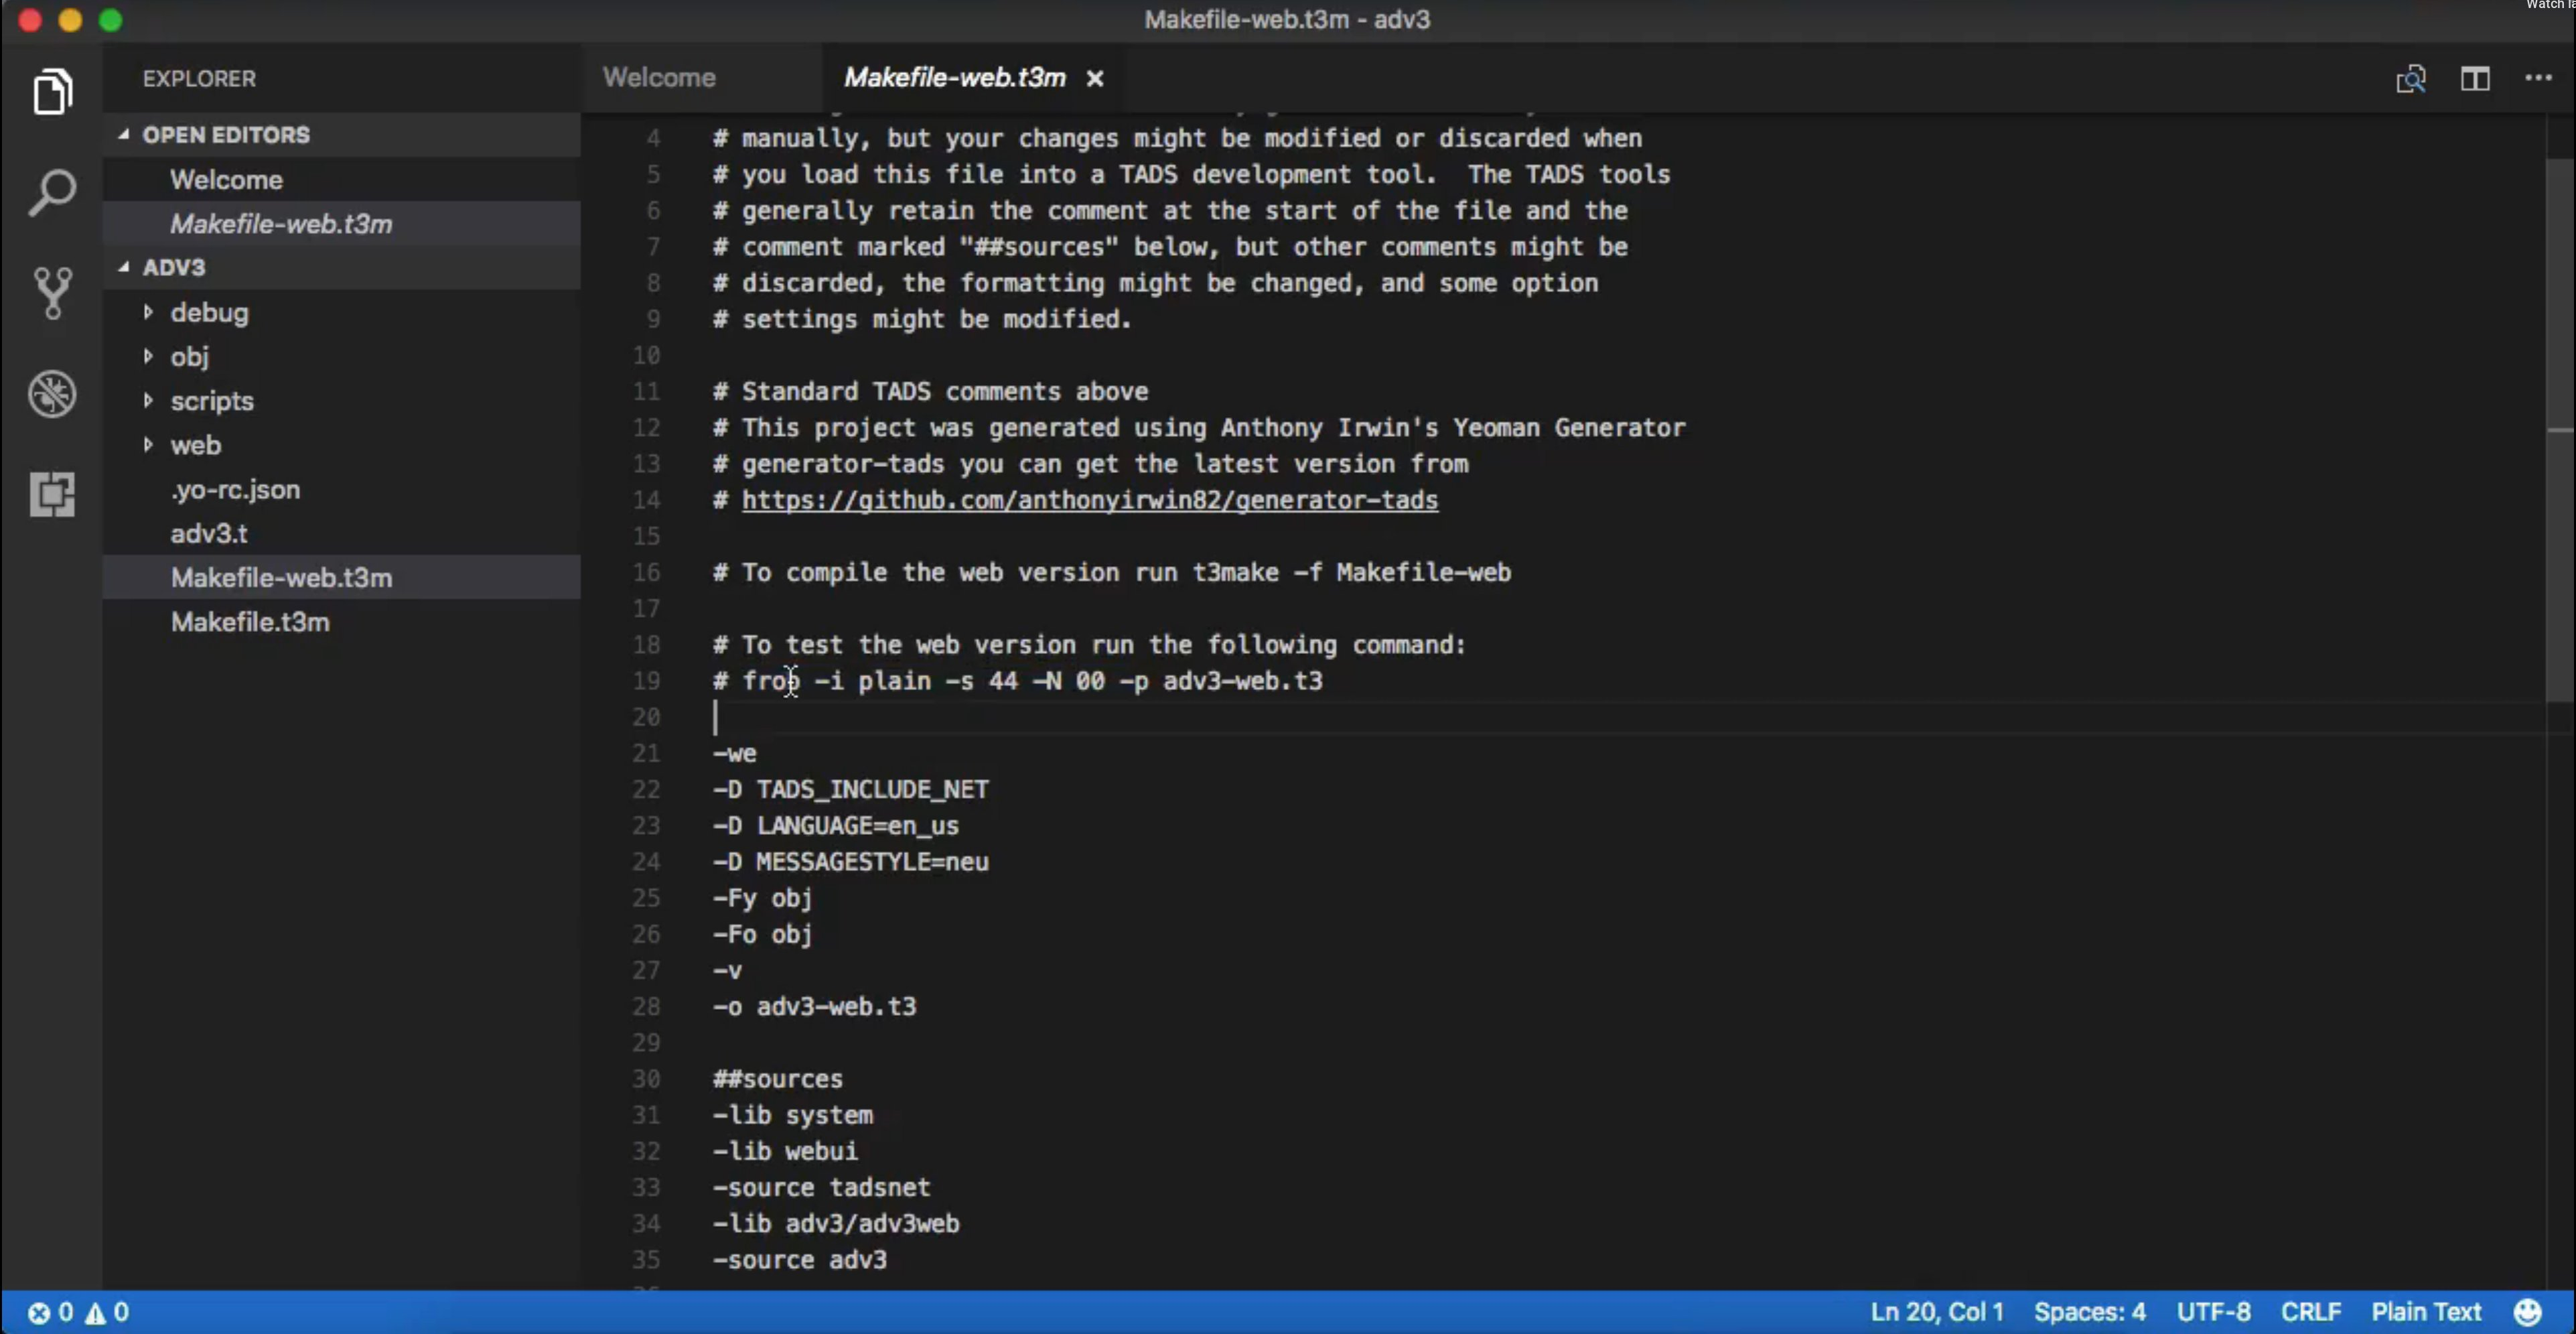
\includegraphics[width=\linewidth]{./media/images/template}\\
  Generator Tads' brief video tutorial makes creating new \textsc{tads3}
  instances easy to learn.}}[-13em]
\subsection{Install Generator Tads using npm}
Notice the \texttt{-g} switch in the \textsc{npm} command. This indicates that we wish to
install \textsc{generator tads} globally but a local instance may be installed
as well.

\begin{lstlisting}
  sudo npm install -g generator-tads
 > spawn-sync@1.0.15 postinstall /usr/lib/node_modules/generator-tads/node_modules/spawn-sync
> node postinstall

+ generator-tads@1.0.2
added 209 packages from 114 contributors in 10.307s
\end{lstlisting}
Create a project directory. This directory may be anywhere you like. I've used
the \texttt{/home/cstevens/doc/gps} directory for this example:

\begin{lstlisting}
  mkdir /home/cstevens/doc/gps
  cd /home/cstevens/doc/gps
\end{lstlisting}
Once you're in the directory, simply run \textsc{yo} to be greeted with a
walkthrough for creating a new project.
\begin{lstlisting}
  yo tads
\end{lstlisting}
If everything worked out alright you will be greeted with this welcome screen
\begin{verbatim}

     _-----_
    |       |    ╭──────────────────────────╮
    |--(o)--|    │ Welcome to the wonderful │
   `---------´   │      tads generator!     │
    ( _´U`_ )    ╰──────────────────────────╯
    /___A___\   /
     |  ~  |
   __'.___.'__
 ´   `  |° ´ Y `

? What type of application do you want to create?
> adv3 Application
  adv3Lite Application
\end{verbatim}
Be certain to select the first option, \texttt{adv3 Application} as the
\textsc{adv3lite} library does not have the features required for embedding web
scripts into your work of \textsc{if}.
NOTE: The project's HTML description cannot contain  at least the ' character.

The system will ask you a few things about your story
\begin{lstlisting}
? What type of application do you want to create? adv3 Application
? Project Name: Cannot contain  / : * ? " < > | or <space> characters. This is the project filename. gps
? Authors Name D. Cooper Stevenson
? Authors Email Address cooper@discdigest.xyz
? The Title of your interactive fiction game GPS Enabled Interactive Fiction
? The Text description of your interactive fiction game Explorers experience the fabric of their surroundings as they may now engage in their environment fully. Your mobile device serves as a gateway to this area's history, biology, wildlife, and archi tecture. Several challenges await, are you ready?
? The HTML description of your interactive fiction game Explorers experience the fabric of their surroundings as they may now engage in their environment fully. Your mobile device serves as a gateway to this areas history, biology, wildlife, and architecture. Several challenges await, are you ready? 
? The IFID for your interactive fiction game. This must be unique for each game the same way as an ISBN is unique for each boo k. You can get an IFID at http://www.tads.org/ifidgen/ifidgen 478AF834-3D02-4B86-9708-88B9572ED8AF   
? The root path to third-party extensions like adv3Lite: Do not add a trailing / E.g. ../extensions ../extensions
   create gps.t
   create Makefile.t3m
   create Makefile-web.t3m
\end{lstlisting}
Let's compile the template
\begin{lstlisting}
t3make
TADS Compiler 3.1.3  Copyright 1999, 2012 Michael J. Roberts
        Files to build: 5
        symbol_export gps.t -> obj/gps.t3s
        compile gps.t -> obj/gps.t3o
        link -> gps.t3p
        preinit -> gps.t3
        add_resources -> gps.t3
        + GameInfo.txt (GameInfo.txt)
\end{lstlisting}
Now we can run the game
\begin{lstlisting}
frob gps
\end{lstlisting}
\begin{figure*}[h]                                                           
 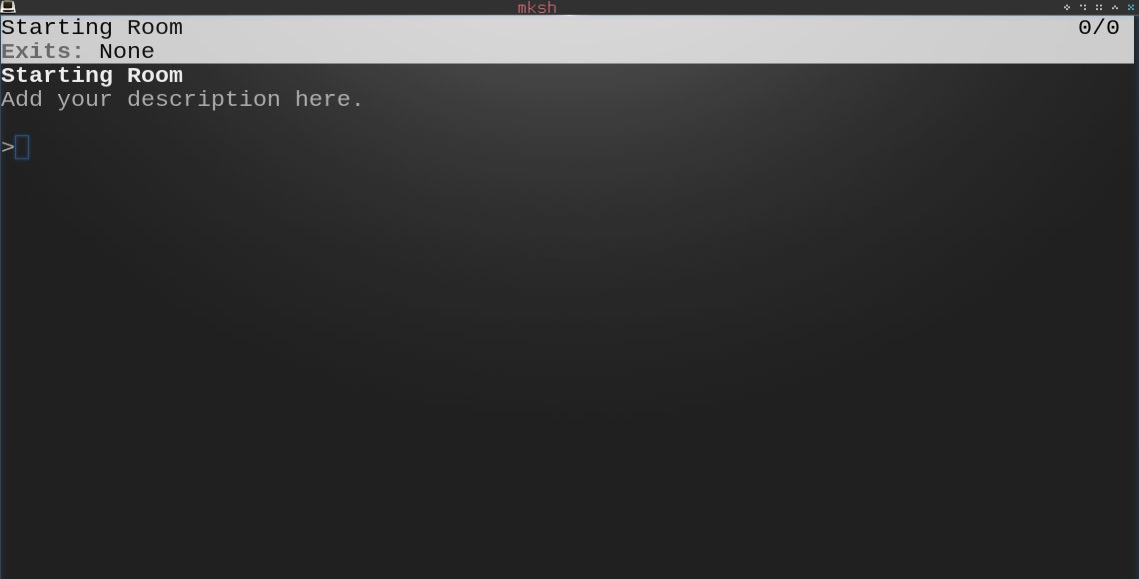
\includegraphics[width=\linewidth]{./media/images/new_text_game.pdf}%
  \scriptsize{\textsc{\\After answering a few questions} about your work of
    Interactive Fiction and compiling  you're greeted with a fresh
    \textsc{tads3} instance running through the \textsc{frob} interpreter.}
  \label{fig:new_text_game}%                                                 
\end{figure*}                                                                
\subsection{compiling a web instance}
\begin{lstlisting}
t3make -f Makefile-web
\end{lstlisting}
Running the instance is simply a matter of running
\begin{lstlisting}
frob -i plain -s 44 -N 00 -p gps-web.t3
\end{lstlisting}
Click on the resulting \textsc{connectwebui} link. A web browser (or new tab)
will appear with your new web\textendash based instance. Let's add some introductory text and a description for the initial area of exploration. The text that follows are excerpts in Chapter 10 of from John L. Stephens' \emph{Incidents of Travel in Yucatan}.
\marginnote{\href{http://www.gutenberg.org/files/33129/33129-h/33129-h.htm}{John L. Stephens' Incidents of Travel in Yucatan}}[-2em]
In \texttt{gps.t} we'll start
with modifying the character set to \textsc{utf-8} (we're civilized people after all) and the \texttt{GameMainDef} function as follows
\begin{lstlisting}
#charset "UTF-8"
...
gameMain: GameMainDef {
    initialPlayerChar = me
    showIntro() {
	"<center><img src='https://web.archive.org/web/20131004041019if_/http://www.gutenberg.org/files/33129/33129-h/images/p165_8.png' width='100%' align='center'></center>
	 <p>
	 <p>";
    }
}
\end{lstlisting}
\begin{figure*}[h]                                                           
 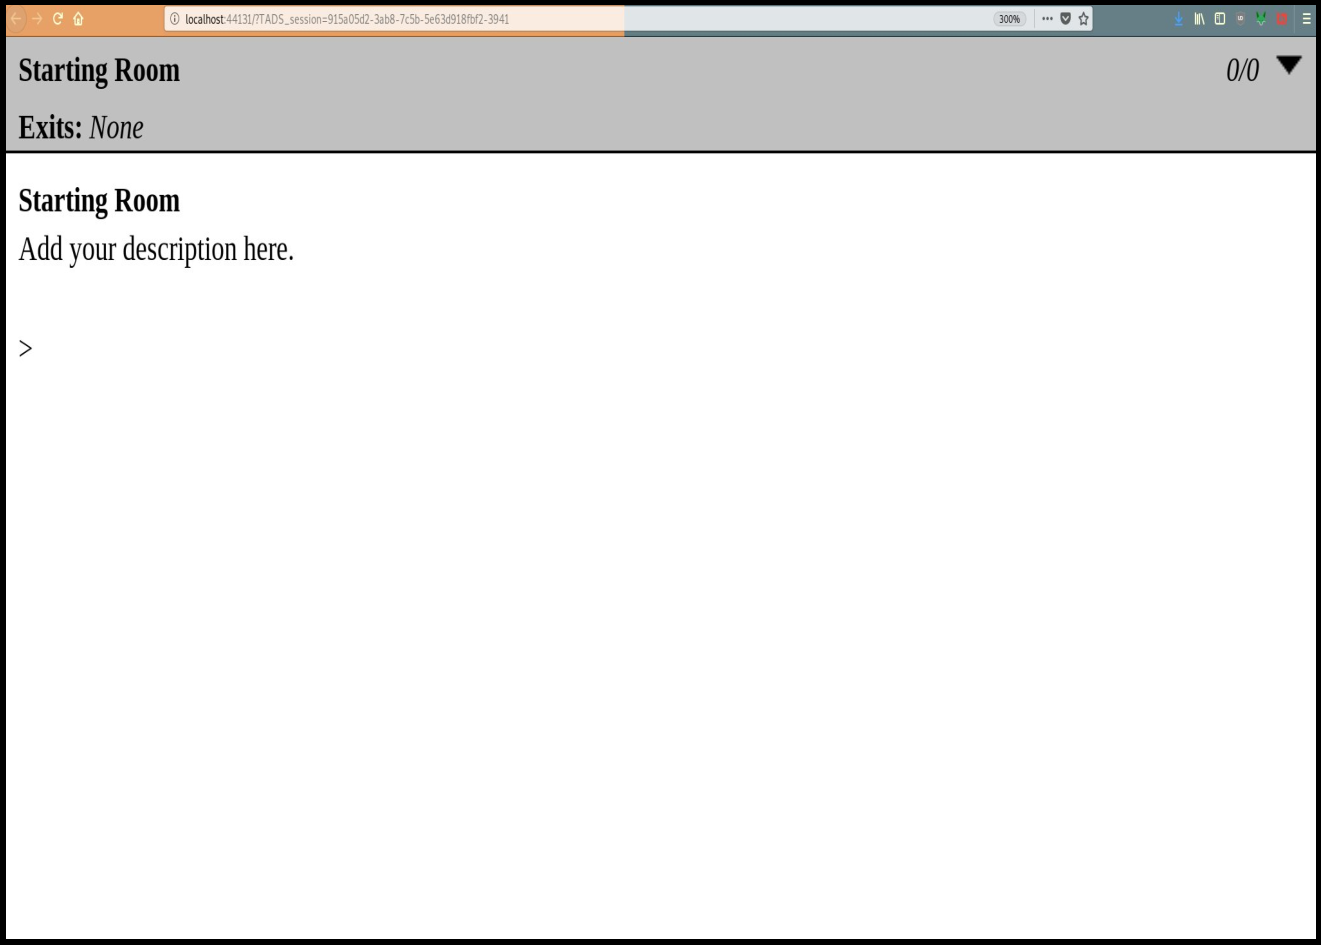
\includegraphics[width=\linewidth]{./media/images/new_web_game.pdf}%
  \scriptsize{\textsc{\\The foundation is now laid } for both a web and
    text\textendash based work of \textsc{if}}
  \label{fig:new_web_game}%                                                 
\end{figure*}
Notice the \texttt{<img src='https://...>} tag in the
\texttt{\scriptsize{showIntro}} function.
\textsc{tads3} allows you to inject \textsc{html, css, and javascript} code
directly into your prose or as a separate library file as we'll see with the
\textsc{gps} process we'll run in the background. If you compile your simulation
for text mode\textemdash handy for concentrating on your writing\textemdash the
compiler will simply ignore these directives and run the
console version. 

Let's add some text to the first area and add an additional area to the
Southeast. First, modify \texttt{gps.t} with an updated room name and a
connection to the Southeast Facade to the Southeast:

\begin{lstlisting}
firstRoom: Room 'Noble Courtyard'
"Among my many causes of regret for the small scale on which I am obliged to present these drawings, none is stronger than the consequent inability to present, with all their detail of ornament, the four great façades fronting this courtyard. There is but one alleviating circumstance; which is, that the side most richly ornamented is so ruined that, under any circumstances, it could not be presented entire."

northeast = se_facade
\end{lstlisting}
Second, let the compiler know about the \texttt{se\_facade} area we're adding by
editing \texttt{Makefile.t3m} (for the console version) and
\texttt{Makefile-web.t3m} (for the web version) as follows:

\begin{lstlisting}
## rooms
-source src/rooms/se_facade/se_facade
\end{lstlisting}

The \texttt{-source} directive tells the compiler where it can expect to find
the resources referenced by each fascet of your project. the \texttt{northeast =
se\_facade} line in \texttt{gps.t} above, for example, tells the compiler that it
should expect a \texttt{se\_facade.t} file somewhere within the project. The
\texttt{-source} directive with corresponding file location is all we need for
the compiler to find the source code, compile into objects, and link the objects
into a single project executable.

Note we've created a \texttt{\scriptsize{src/rooms}} subdirectory with an additional
subdirectory for the \texttt{\scriptsize{se\_facade}} area to illustrate good housekeeping
while building the project. Good organization practices early pay off
dividends as the project grows.

The Southeast Façade's \texttt{\scriptsize{(src/rooms/se\_facade/se\_facade.t)}} code looks like this:

\begin{lstlisting}
  
#charset "utf-8"
#include <adv3.h>
#include <en_us.h>

se_facade: Room 'Southeast Façade'


"This façade is on the left of the visiter entering the courtyard. It is one hundred and seventy-three feet long, and is distinguished by two colossal serpents entwined, running through and encompassing nearly all the ornaments throughout its whole length. The two plates which follow represent the only parts remaining."

southwest = firstRoom
  ;
\end{lstlisting}
Overall, we have these steps for making our basic \textsc{if} framework:
\begin{itemize}[leftmargin=0em]
  \item{Change the default character set to \textsc{utf-8}}
  \item{Add introductory and description text to the main file to \texttt{\scriptsize{(gps.t)}}}
  \item{Create a connector \texttt{\scriptsize{(northeast = se\_facade)}} to \texttt{\scriptsize{gps.t}}}
  \item{Create a \texttt{\scriptsize{se\_facade.t}} file with connector back to
      \texttt{\scriptsize{firstRoom}} \texttt{\scriptsize{(southwest = firstRoom)}}}
  \item{Tell the Make files \texttt{\scriptsize{(Makefile.t3m}} and
        \texttt{\scriptsize{Makefile-web.t3m)}} about the new area {\texttt{se\_facade}}}
  \end{itemize}
With these additions we are greeted with a working two\textendash area project viewed through the eyes of an explorer in 1848:
%\pagebreak
\begin{figure*}[ht]                                                           
  \begin{center}
 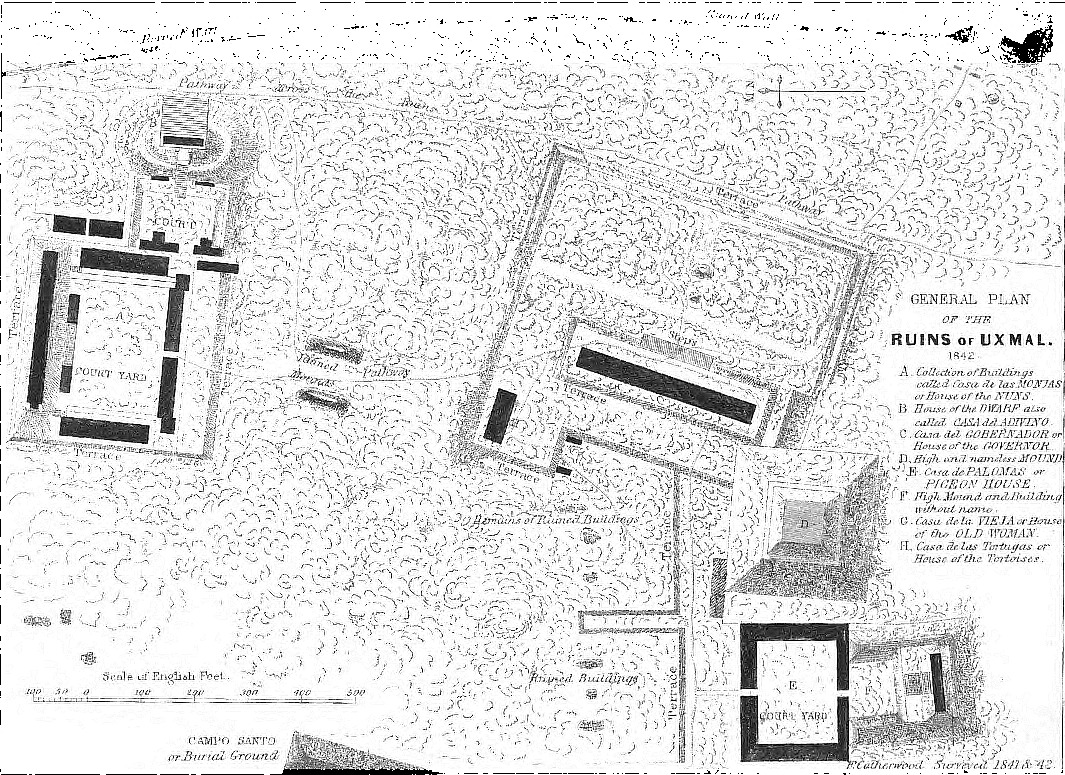
\includegraphics[width=\linewidth]{./media/images/if_cover}%
  \label{fig:if_cover}%                                                 
  \end{center}
\end{figure*}
\smallbreak
\noindent \textbf{\large{\emph{Incidents of Travel in Yucatan}}}
\smallbreak
\noindent Passing through the arched gateway, we enter a noble courtyard, with four great façades looking down upon it, each ornamented from one end to the other with the richest and most intricate carving known in the art of the builders of Uxmal; presenting a scene of strange magnificence, surpassing any that is now to be seen among its rains. This courtyard is two hundred and fourteen feet wide, and two hundred and fifty-eight feet deep. At the time of our first entrance it was overgrown with bushes and grass, quails started up from under our feet, and, with a whirring flight, passed over the tops of the buildings. Whenever we went to it, we started flocks of these birds, and throughout the whole of our residence at Uxmal they were the only disturbers of its silence and desolation. 
\smallbreak
\noindent \textbf{\emph{Courtyard Entrance}}
\smallbreak
\noindent Among my many causes of regret for the small scale on which I am obliged to present these drawings, none is stronger than the consequent inability to present, with all their detail of ornament, the four great façades fronting this courtyard. There is but one alleviating circumstance; which is, that the side most richly ornamented is so ruined that, under any circumstances, it could not be presented entire.
\smallbreak
\noindent \textbf{\emph{>ne}}
\smallbreak
\noindent \textbf{\emph{Southeast Façade}}
\smallbreak
\noindent This façade is on the left of the visiter entering the courtyard. It is one hundred and seventy-three feet long, and is distinguished by two colossal serpents entwined, running through and encompassing nearly all the ornaments throughout its whole length. The two plates which follow represent the only parts remaining.
\smallbreak
\noindent \textbf{\emph{>}}
% \subsection{creating a base tads3 system}
\subsection{pull tads3 javascript extension}
The ability to write inline Javascript into \textsc{tads3} code is handled by
Ben Cressey's excellent webscrptres
extension.\marginnote{\href{https://bitbucket.org/bcressey/t3ext}{Ben Cressey's
    webscrptres extension}} The extension may by dowloaded as a compressed
archive or may be 'pulled' from the source repository. The repository may be
pulled either to your local project directory
(\texttt{/home/cstevens/doc/gps/lib} in this case) or globally. This example
installs Cressey's extensions globally as it is convenient for future builds.
You will have to remember to re\textendash pull the extension for each new work
you create. Localized extensions, however, prevents potential versioning
problems and keeps your projects self\textendash contained:
\begin{lstlisting}
  cd /usr/local/share/frobtads/tads3/lib
  sudo sudo git clone https://bitbucket.org/bcressey/t3ext.git 
\end{lstlisting}
The repository will now be cloned to
\begin{lstlisting}
/usr/local/share/frobtads/tads3/lib/t3ext
\end{lstlisting}
\subsection{modify Makefile-web.t3m}
Make sure \texttt{\scriptsize{adv3/adv3web}} is defined prior to
\texttt{\scriptsize{t3ext/webui/webscript}} to avoid webscript's ``initDisplay''
object being loaded before \textsc{tads3}'s base \textsc{adv3web}. The compiler
will issue an error to this effect if the base library is not loaded before the
\textsc{webscript} library is loaded. Here is
\texttt{\scriptsize{Makefile-web.t3m}} in it's entirety:
\begin{lstlisting}
# Standard TADS comments above
# This project was generated using Anthony Irwin's Yeoman Generator
# generator-tads you can get the latest version from
# https://github.com/anthonyirwin82/generator-tads

# To compile the web version run t3make -f Makefile-web

# To test the web version run the following command:
# frob -i plain -s 44 -N 00 -p gps-web.t3

-we
-D TADS_INCLUDE_NET
-D LANGUAGE=en_us
-D MESSAGESTYLE=neu
-Fy obj
-Fo obj
-v
-o gps-web.t3

##sources
-lib system
-lib webui
-lib adv3/adv3web
# javascript hook
-lib t3ext/webui/webscript

-source tadsnet
-source gps

## rooms
-source src/rooms/se_facade/se_facade

## gps daemon
-source lib/gps_daemon.t

-res
GameInfo.txt
\end{lstlisting}
\section{enabling gps}
\begin{itemize}[leftmargin=0em]
\item From your base directory (\texttt{\scriptsize{/home/cstevens/doc/gps}} in this case), create a '\texttt{lib}'
(*nix parlance for supporting libraries) directory
\begin{lstlisting}
  mkdir /home/cstevens/lib/
\end{lstlisting}
\item Create a file called \texttt{\scriptsize{gps\_daemon.t}} under the \texttt{lib} directory with the contents listed below. This code contains the correct
  \textsc{gps} coordinates for our two locations and the system should thus
  compile. We'll review how to find and test the coordinates in the
  \emph{Finding GPS Coordinates} section on page \pageref{sec:coordinates} and
  the \emph{Testing} section on page \pageref{sec:testing}.
  \marginnote{GPS daemon code for passing client\textendash browser GPS
    information to \textsc{tads3}}[2em]
\begin{lstlisting}
#charset "utf-8"
#include <adv3.h>
#include <en_us.h>
#include <bignum.h>

DefineIAction(GPS);

VerbRule(GPS)
        'gps'
        :  GPSAction
        verbPhrase = 'script/scripting'
;

#define JS(STR, ARGS...) JavaScript.eval( ## #@STR ##, ##ARGS ## )
modify GPSAction
    execAction()
{
        JS({

var options = {
    enableHighAccuracy: true,
    timeout: 5000,
    maximumAge: 30000 
};

function success(pos) {
    serverRequest("/webui/gpsEvent?lat=" + pos.coords.latitude
        + '&lon=' + pos.coords.longitude + '&acc=' + pos.coords.accuracy);
    console.log('lattitude: ' + pos.coords.latitude + ' longitude: ' + pos.coords.longitude + ' Accuracy: ' + pos.coords.accuracy);
};

function error(err) {
    console.warn('ERROR(' + err.code + '): ' + err.message);
};

navigator.geolocation.watchPosition(success, error, options);

        });
    }
;

// This is TADS3 Code
gpsEvent: WebResource
    vpath = '/webui/gpsEvent'

    processRequest(req, query)
    {
            /* Do something... */
            //note the limiting place number to 'loosen' range in lat/lon
            local latitude = new BigNumber('<<query['lat']>>',7);
            local longitude = new BigNumber('<<query['lon']>>',7);
            //turn the lat & lon into a string for case statement below
            local location = toString([latitude,longitude]);
            "<p>location: <<location>>   lat: <<latitude>>  lon: <<longitude>></p>";

            // switch(latitude,longitude)
            switch(location)
            {
              /* Courtyard Entrance */
            case ('20.3608,-89.7707'):
              if (me.isIn(firstRoom) == nil)
                {
                  me.scriptedTravelTo(firstRoom); 
                  /* send a new prompt */
                  commandWin.write('<br />&gt; '); 
                  commandWin.flushWin();

                  /* set the UI state */
                  commandWin.mode = 'inputLine';
                  commandWin.isInputOpen = true;

                  /* send the inputLine event to the client */
                  commandWin.sendWinEvent('<inputLine/>');
                } //end me.location
            break;
              /* Southeast Facade */
              case ('20.3612,-89.7709'): 
              if (me.isIn(se_facade) == nil)
                {
                me.scriptedTravelTo(se_facade);
                /* send a new prompt */
                commandWin.write('<br />&gt; '); 
                commandWin.flushWin();

                /* set the UI state */
                commandWin.mode = 'inputLine';
                commandWin.isInputOpen = true;

                /* send the inputLine event to the client */
                commandWin.sendWinEvent('<inputLine/>');
                } //end me.location
              break;
            default:
             {
                /* set the UI state */
                commandWin.mode = 'inputLine';
                commandWin.isInputOpen = true;

                /* send the inputLine event to the client */
                commandWin.sendWinEvent('<inputLine/>');

             }
         }
        sendAck(req);
    }
;
\end{lstlisting}
\end{itemize}
Notice that the \textsc{gps} daemon code is actually written in \textsc{tads3}
with embedded Javascript. After the header include statements we'll define a new
\textsc{tads3} verb called \texttt{gps}.
\begin{lstlisting}
DefineIAction(GPS);

VerbRule(GPS)
        'gps'
        :  GPSAction
        verbPhrase = 'script/scripting'
;
\end{lstlisting}
The next line tells \textsc{tads3} that anytime it sees the \texttt{\scriptsize{JS()}}
directive that it should be passed to the browser for direct processing. The
power here lies in the ability for the directive to pass variables
back\textendash and\textendash forth to the \textsc{tads3} compiler.
\begin{lstlisting}
#define JS(STR, ARGS...) JavaScript.eval(## #@STR ##, ##ARGS ##)
\end{lstlisting}
The \texttt{\scriptsize{modify GPSAction}} defines the action that should be taken when the
\texttt{gps} command is executed. In this case the command initiates the
browser's client\textendash side \textsc{gps} subsystem with the Javascript code that
immediately follows, ie., the statements enclosed in the \texttt{\scriptsize{JS\{(...)\}}} directive.

The actual accumulation of the Interlocutor's position is collected via the
sparsely named \texttt{lat} and \texttt{lon} variables. The command also
provides an accuracy variable (\texttt{acc}) that you may use for testing or as
a part of an expanded subroutine to ensure that your positional data is correct.
\marginnote{The polling loop queries the Interlocutor's \textsc{gps} device
  every five seconds producing position variables for processing}[2em]
\begin{lstlisting}
    serverRequest("/webui/gpsEvent?lat=" + pos.coords.latitude
        + '&lon=' + pos.coords.longitude + '&acc=' + pos.coords.accuracy);
\end{lstlisting}
Amazingly we return to \textsc{tads3} code where the \textsc{javascript} \textsc{lat/lon}
variables are passed as an array for assignment back into \textsc{tads3}
\begin{lstlisting}
 local latitude = new BigNumber('<<query['lat']>>',7);
 local longitude = new BigNumber('<<query['lon']>>',7);
\end{lstlisting}
The \texttt{\scriptsize{latitude}} and \texttt{\scriptsize{longitude}} numbers are cut to give a slightly
wider range of positions (within 10 meters or so) accepted to create an event
that the Interlocutor has actually entered the area of interest. The variables
are now converted into a text string for testing by a \texttt{\scriptsize{case}} statement
later on and a print statement is added for use during development.
\begin{lstlisting}
local location = toString([latitude,longitude]);
"<p>location: <<location>>   lat: <<latitude>>  lon: <<longitude>>
</p>";
\end{lstlisting}
Once matching pair of coordinates are received a \textsc{tads3} \texttt{\scriptsize{me.scriptedTravelTo}} event is triggered.
\begin{lstlisting}
/* Southeast Facade */
case ('20.3612,-89.7709'): 
  if (me.isIn(se_facade) == nil)
  {
    me.scriptedTravelTo(se_facade);
  ...
\end{lstlisting}
\marginnote{\href{http://www.tads.org/howto/t3npcTravel.htm}{scriptedTravelTo
    details from the \textsc{tads3} Howto guide}}[1em]
Notice that a \emph{scripted} event is triggered. The \texttt{\scriptsize{scriptedTravelTo()}} method
always carries out a single nested action, which means that it does everything
that would normally happen when the Interlocutor moves into this location. This
includes any narration, travel connector descriptions, tripped events beyond
location, etc. An exciting possibility that immediately comes to mind is a work
where a 'bonus' location isn't overtly stated; one that is only inferred by clues
found elsewhere. When the Interlocutor approaches the 'secret' location an
entire story line opens up.
\marginnote{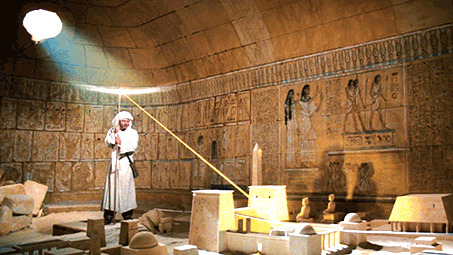
\includegraphics[width=\linewidth]{./media/images/indie}%
  \label{fig:indie}\\ Locations inferred only through clues found elsewhere
}[-6em]
Finally, these lines perform some house cleaning after the location change by
resetting the \textsc{ui} state and preparing the parser for input.
\begin{lstlisting}
/* set the UI state */
commandWin.mode = 'inputLine';
commandWin.isInputOpen = true;

/* send the inputLine event to the client */
commandWin.sendWinEvent('<inputLine/>');
\end{lstlisting}
\subsection{finding gps coordinates}
  \label{sec:coordinates}%                                                 
\begin{figure*}[h]                                                           
 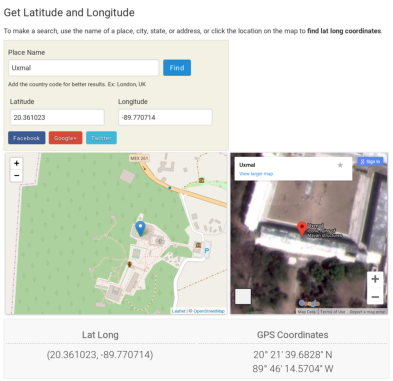
\includegraphics[width=\linewidth]{./media/images/lat_lon.pdf}%
  \scriptsize{\textsc{\\Getting Latitude and Longitude coordinates} is
    straight\textendash forward using \textsc{latlon.net}.}
  \label{fig:lat_lon}%                                                 
\end{figure*}
\begin{figure*}[h]                                                           
 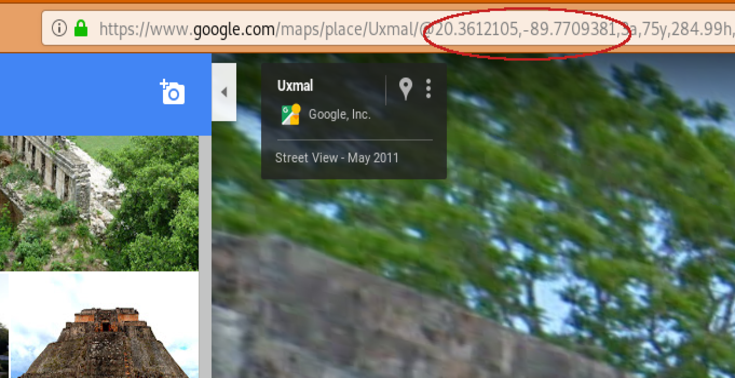
\includegraphics[width=\linewidth]{./media/images/url.pdf}%
  \scriptsize{\textsc{\\Reading the lat/lon} coordinates from Google maps}
  \label{fig:facade}%                                                 
\end{figure*}
\marginnote{\href{https://www.latlong.net/}{latlong.net gives geographic
    coordinate information through a Google Maps interface}}
\noindent At least two methods exist for zeroing in your \textsc{if} geography's
\textsc{gps} coordinates. The first is through \textsc{latlong.net}; the second
involves reading the \textsc{url} line from Google Maps. \textsc{latlong.net} provides a map and satellite view opposite each other. The coordinates you need
for entry into the \textsc{if gps} system are listed below on the left hand
side. Once you've established your initial position you can use Google Maps
street view to each position and quickly read off the lat/lon entries in your
current position's \textsc{url} status line.
\begin{figure*}[h]                                                           
 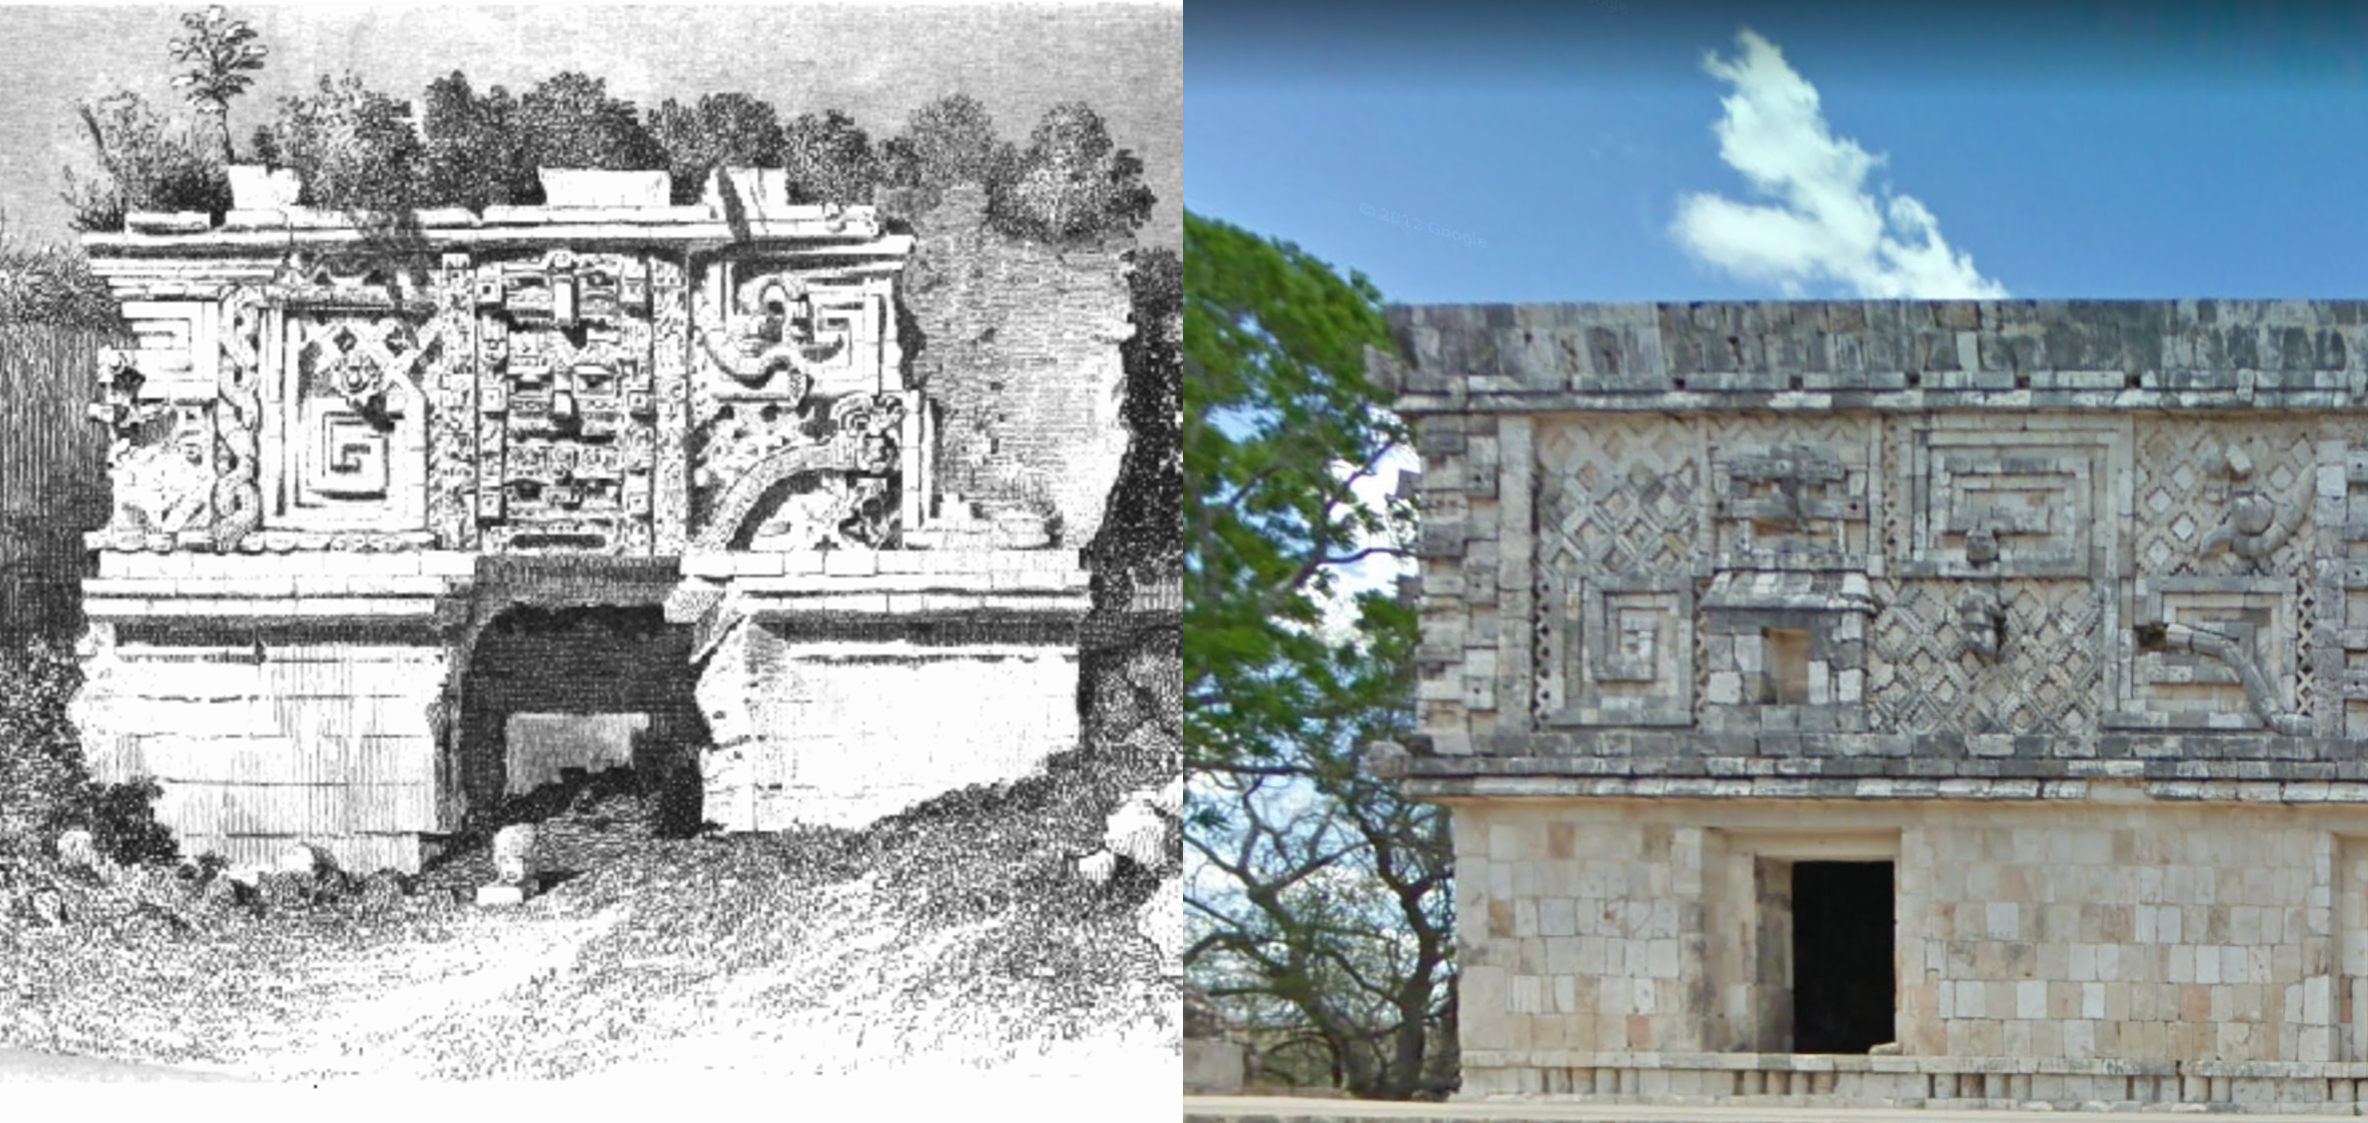
\includegraphics[width=\linewidth]{./media/images/court_facade.pdf}%
  \scriptsize{\textsc{\\Façade of the Monjas sketch} from \emph{circa} 1848 shown beside the Façade today}
  \label{fig:facade}%                                                 
\end{figure*}
\section{testing}
\label{sec:testing}
Once you've compiled your draft \textsc{if} with each area's respective \textsc{gps}
coordinates you'll need to test each location to ensure that the system works
when the browser sends a pair of coordinates that match one of your designated
sites. This is achieved using the browser's \textsc{about:config} options to
manually change the browser's reported latitude and longitude coordinates. Once
the browser is set up to modify it's coordinate reporting testing your testing
is mostly a matter of organization to ensure that each position is checked for
accuracy and completeness.

\marginnote{\href{https://www.comparitech.com/blog/vpn-privacy/change-location-chrome-firefox-spoof/}{Detailed description for changing your browser's reported position using the browser's \textsc{about:config conf} configuration parameters}}
Several browser plugins exist to ``spoof'' your browser's reported position. No
plugin I've tested to date works correctly; even though the coordinates appear
to be modified by the plugin the system at the reporting level the \textsc{Javascript}
code pulls from the \textsc{gps} coordinates of your location's nearest central
office \textsc{(co)} location.

Testing involves the following steps:
\begin{itemize}[leftmargin=0em]
  \item{Modify the browser's configuration to point to the location you wish to
      test}
  \item{Compile and run your \textsc{if}prototype}
    \end{itemize}
\begin{itemize}[leftmargin=0em]
\item{Open a new tab in your browser and type the command \texttt{\scriptsize{about:config}}
    in your browser and agree that you understand that manually changing the
    configuration ``may void your warranty''}
\item{Search for the \texttt{geo.wifi.uri} parameter}
  \item{modify the \textsc{json} object to the coordinates listed in an
      adjacent area in the prototype (the \texttt{\scriptsize{se\_facade}}
      located at \texttt{\scriptsize{lat 20.3612 lon -89.7709}} in this case)}
\end{itemize}
  \begin{lstlisting}
    data:application/json,{"location": {"lat": 20.3612, "lng": -89.7709}, "accuracy": 1.0}
  \end{lstlisting}
\begin{figure*}[h]                                                           
 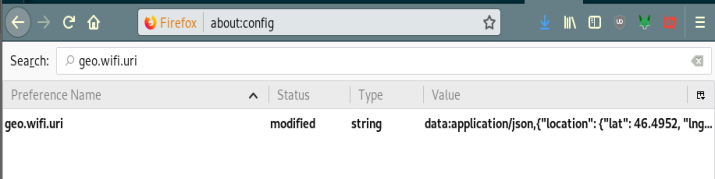
\includegraphics[width=\linewidth]{./media/images/gps_config.pdf}%
  \scriptsize{\textsc{\\Using the browser's geo.enabled} parameter in the
    browser configuration dialog ()}
  \label{fig:about_config}%                                                 
\end{figure*}
\subsection{compiling and running your prototype}
\begin{itemize}[leftmargin=0em]
\item{compile your \textsc{if} prototype with the \textsc{t3make} command}
\begin{lstlisting}
t3make -a -f Makefile-web.t3m
\end{lstlisting}
\item{Next, run the \textsc{frobtads} interpreter and click the resulting link}
\begin{lstlisting}
frob -i plain -s 44 -N 00 -p gps-web.t3

connectWebUI:http://localhost:40241/?TADS_session=680c40b7-bd92-04e6-297af4b44661-61c2
\end{lstlisting}
\item{Enter the \texttt{gps} command at your \textsc{if} instance's parser command prompt to initiate the \textsc{gps} daemon}
\begin{lstlisting}
  gps
\end{lstlisting}
\item{Permit the browser to access your location from the browser's pop\textendash up dialog box.}
\end{itemize}
You should now see the location service working anytime you execute a parser
command. The environment looks similiar to this (the Courtyard Entrance description is truncated):
\begin{quote}
  \textbf{\emph{Courtyard Entrance}}
  
Among my many causes of regret for the small scale on which I am obliged to
present these drawings, none is stronger than the consequent inability to
present, with all their detail of ornament, the four great façades fronting this
courtyard.
\smallskip

\textbf{\emph{>gps}}
\smallskip

Nothing obvious happens.
\smallskip

\textbf{\emph{>look}}
\smallskip

location: 46.4952,-124.0508 lat: 46.4952 lon: -124.0508 
\end{quote}
The location as a string along with the \texttt{lat} and \texttt{lon} variables
are printed for debugging. This may be changed for production by commenting out
the following lines in \texttt{\scriptsize{gps\_daemon.t}}.

\begin{lstlisting}
"<p>location: <<location>>   lat: <<latitude>>  lon: <<longitude>></p>";
\end{lstlisting}
After a few moments you should see your location change; you may need to refresh
your browser depending on your browser's settings and enabled plugins. 
\begin{figure*}[h]                                                           
\hspace*{-1.75cm} 
 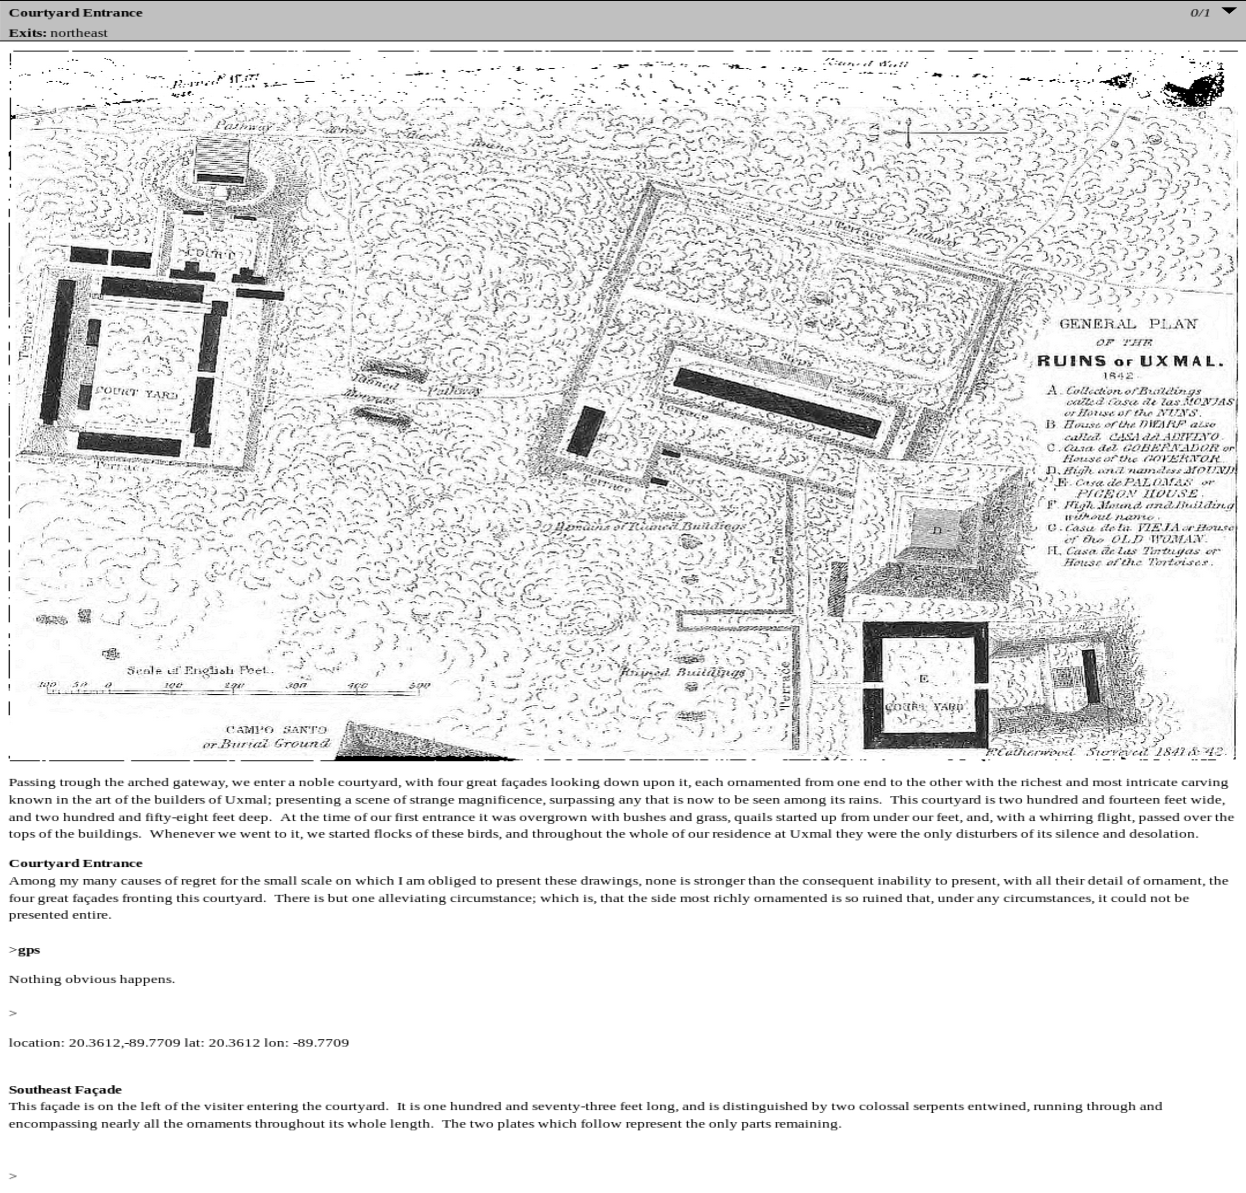
\includegraphics[width=0.9\paperwidth]{./media/images/switch.pdf}%
  \scriptsize{\textsc{\\Finished product depicting} the triggered site change
    when the browser reports coordinates matching the work's location}
  \label{fig:switched}%                                                 
\end{figure*}

% * Testing: spoof geo in browser
%   ** geo-spoofing plugins do not work.
%   ** Changing geo point in browser:
% https://www.comparitech.com/blog/vpn-privacy/change-location-chrome-firefox-spoof/
%This is a test ov figuring out why this thing is so weird.

% * Also need to refresh the page after testing.
% \reversemarginpar\marginnote{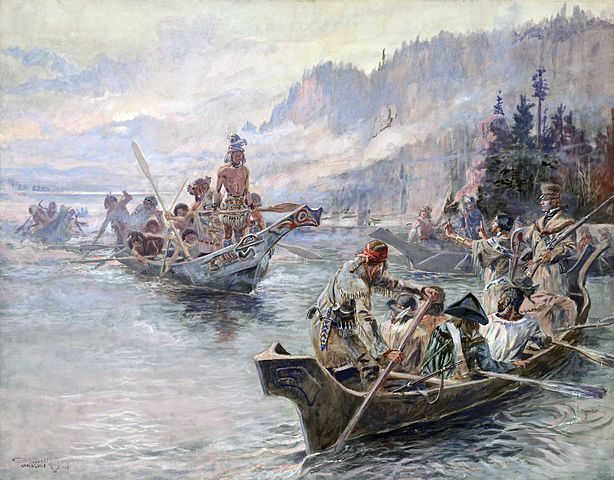
\includegraphics[width=\linewidth]{./media/images/lewis}\href{https://www.youtube.com/watch?v=NJarxpYyoFI}{\\This is the marginnote caption(linked)}}


 \chapter*{}
  \begin{textblock*}{70.9mm}(0mm,0mm)
    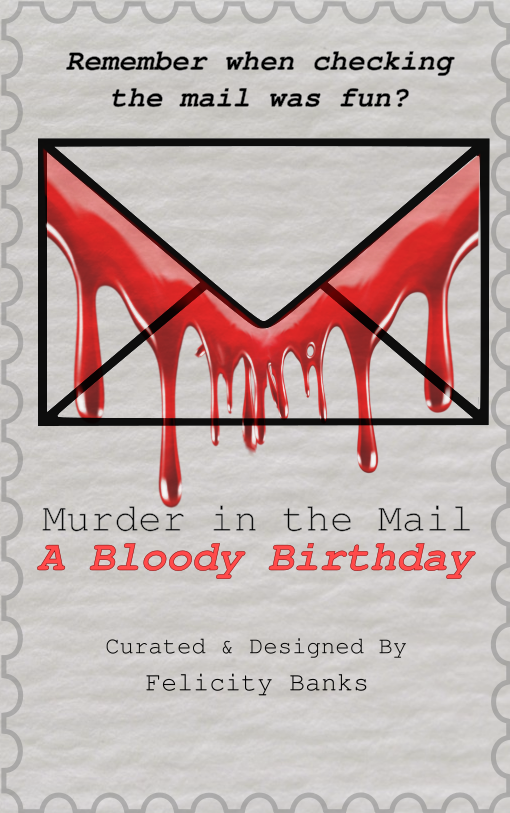
\includegraphics[width=\paperwidth]{./media/images/murder_ad}
  \end{textblock*}
  \chapter{Murder In The Mail\\ \small{Remember When Checking the Mail Was Fun?}}
 \label{sec:murder}
 \begin{figure*}[h]                                                           
 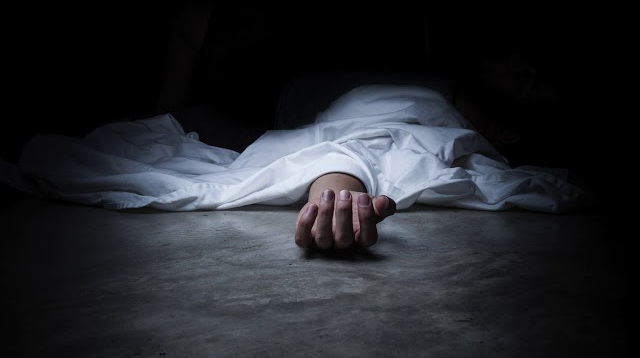
\includegraphics[width=\linewidth]{./media/images/murder}%
%  \scriptsize{\textsc{\\This is} the article main image caption.}
  \label{fig:editorial}%                                                 
\end{figure*}                                                                
\begin{quotation} 
\noindent\color{Sepia}{{\textit{\textbf{“To catch a killer, one must think like a killer”}}}}\\[.5mm]
%remove following line space if you're tight on vertical room and need to fit on
%single page

\hfill\color{Sepia}{\small{\textendash \textsc{Belinda Bauer, The Beautiful Dead}}}
\end{quotation} 
\newpage
Felicity Banks recently published her new work, \emph{Magic in the Mail}.
\emph{Magic} is a ``whodunnit'' where you receive pretty cool stuff, I must say,
through the mail. We exchanged emails for this interview.
\medskip

\emph{Felicity Banks, you've written novels as well as writing for Tin Man Games and others. What made you invent a system as unique as Murder in the Mail and Magic in the Mail?}
\medskip

I've been cheerfully telling other novelists that they can get quite a decent advance for writing IF, and my print publisher (Odyssey Books) asked me to write something interactive that could be part of the new imprint, Publisher Obscura, which is all about picture books for adults. One thing led to another and once I had a solid idea (or three) I was unable to let it go. 

\medskip
\emph{Can you tell us how these stories work?}

\medskip
At present there are two stories, and one in development. I originally chose crime because whodunnit books already have a puzzle element for the canny reader. So in the story Murder in the Mail: A Bloody Birthday, a girl named Naomi is killed at her own birthday party. It's clear that one of her friends is the killer, and they're all artists... so "you" have asked them to send you both their suspicions of one another and their artworks done around the time of the murder.

I hired six artists and six writers, so each character in the story has their own voice and their own artistic style. Every picture contains clues about the identity of the killer (and of course the secrets of the other characters). So it's a sampler of authors and artists as well as a story and a puzzle (although I am too merciful to leave readers unsure of the answers, so it resolves as neatly as a regular book).

In the subscription version of the story (only available in Australia now, sorry) the reader receives a parcel each week containing a letter, a postcard, at least one physical object, and a piece of art. The physical objects are also clues about the killer, and are carefully chosen to involve all the reader's senses.

The story will be converted into a 'normal' book in 2019, so it's only available for a limited time.

\medskip
\emph{You mentioned Magic in the Mail? What's that?}

\medskip
There is a full-length Magic in the Mail story in development that still has a minor puzzle element as well as a wider range of art (a hand-printed silk bookmark and things like that). . . but in the meantime I wrote a Magic in the Mail mini-story called Emmeline's Empire that is a steampunk fantasy love story between two women. It includes jewellery, a castle for the reader to build, and a sing by the Littmus Steampunk Band.

\medskip
\emph{Shut up and take my money!}

\medskip
Okay. The store is at MurderintheMail.net/store.
\bigskip
\marginnote{\href{http://ifdb.tads.org/search?searchbar=Felicity+Banks&searchGo.x=0&searchGo.y=0}{Felicity Banks' Interactive Fiction Database page}}[3em]
\begin{wrapfigure}{l}{0.45\textwidth}
  \vspace{-2em}
  \begin{center}
  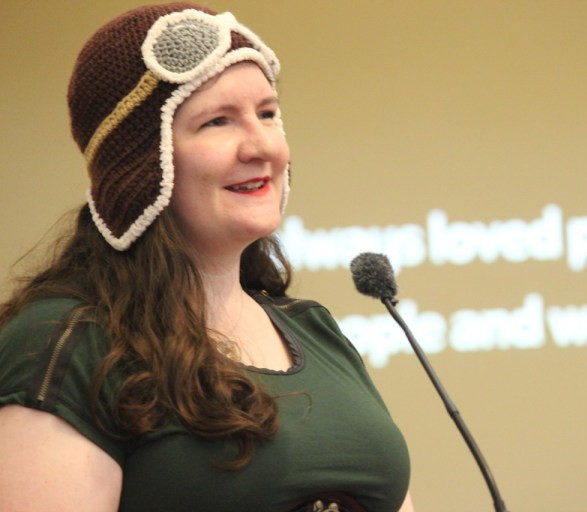
\includegraphics[width=\linewidth]{./media/images/felicity}%
%  \scriptsize{\textsc{\\This is} the article main image caption.}
  \label{fig:brian}%
  \end{center}
\end{wrapfigure}                                                                
\noindent\emph{Felicity Banks has several novels published with Odyssey Books (a small press in
Australia) and is a minion of Tin Man Games (being heavily involved with their
\emph{choices that matter} serial story app on iOS and Google Play) as well as
various other things (all listed on her ifdb page). Felicity's ChoiceScript tale, \emph{Scarlet Sails}, placed 7th in the 2015 IF Comp.}

% \chapter*{}
% \begin{textblock*}{70.9mm}(0mm,0mm)
% \includegraphics[width=\paperwidth]{./media/images/type}
% \end{textblock*}

% \chapter{Epilogue\\ \small{Standing On The Shoulders of Giants}}
% \label{ch:epilogue}
% \input{./epilogue.tex}

% print page notes
% \printpagenotes
\end{document}
% Author's Margin Credit
% \marginnote{\includegraphics[width=\linewidth]{/tmp/felice}\href{https://en.wikipedia.org/wiki/Republic_(Plato)}{\\\\By Felicity Banks}}

% Author's Bio
% \begin{wrapfigure}{l}{.25\textwidth}
%   \vspace{-20pt}
%   \begin{center}
%      \includegraphics[width=0.25\textwidth]{/tmp/felice}
%      \caption*{\href{http://cooper.stevenson.name}{\textit{Felicity Banks}}}
%      % } % end parbox
%     \end{center}
%  \end{wrapfigure} 
%\noindent \textit{Banks’ evocation, and then subversion and manipulation, of small details of Australian colonial history is clever and got me checking (historical) names and details on more than one occasion. The story’s action is fast-paced & drives the plot forward with a precision akin to the machinery it embraces.} \\ \\

